
\chapter{Accelerated array code}
\label{ch:implementation}
\epigraph{The trouble with opportunity is that it always comes disguised as hard work.}%
{\textsc{---herbert v.\ prochnow}}

The previous chapter described the design of the Accelerate language, an
embedded DSL of operations over arrays, rich enough to express some interesting
real-world problems. This chapter details the architecture and implementation of
a backend for parallel execution on CUDA hardware.


\section{Parallel algorithms in CUDA}
\label{sec:parallel_algorithms_in_cuda}

The CUDA architecture is a parallel computing platform and programming model
created by NVIDIA and implemented by the graphics processing units
(GPUs)\index{GPU|see {graphics processing unit}}\index{graphics processing unit}
that they produce. Using CUDA, the GPU becomes accessible not just for
graphics applications, but for computational tasks much like a CPU\@. Unlike
CPUs, however, GPUs have a parallel throughput architecture that emphasises
executing many concurrent threads slowly, rather than executing a single thread
very quickly.
% Unlike CPU cores, instructions are issued in order and there is no
% branch prediction and no speculative execution.
See section~\ref{sec:cuda} for more information.

% The CUDA hardware architecture is built around a scalable array of
% multithreaded \emph{streaming multiprocessors} (SMs).\index{SM|see {streaming
% multiprocessor}}\index{streaming multiprocessor} When a CUDA program on the
% host CPU invokes a \indexe{kernel} --- a function which executes on the GPU
% --- a \emph{grid} of threads grouped into equally sized \emph{blocks} is
% % \index{thread!grid} \index{thread!block}
% enumerated and distributed to the multiprocessors for execution, using a
% \emph{single-instruction, multiple thread} (SIMT) model.\index{SIMT|see {single
% instruction multiple thread}}\index{single instruction multiple thread} The
% multiprocessor creates, manages, schedules, and executes threads in groups of 32
% parallel threads call a \indexe{warp}. All threads in a warp share a single
% program address counter, so divergent threads within a warp are handled via
% predicated execution; for example the positive and negative cases of a branch
% are executed in sequence, with threads not on the current execution path made
% inactive (disabled). In essence, streaming multiprocessors replace the complex
% instruction scheduling logic of a CPU which increases single threaded
% performance --- namely out-of-order execution, branch prediction and speculative
% execution --- with many additional ALUs (arithmetic logic units, often referred
% to as CUDA cores) all executing the same instruction sequence in parallel in
% order to increase total instruction throughput. Details of the CUDA
% architecture can be found in the CUDA C programming
% guide~\cite{NVIDIA:2012wf}; we present only those features required for the
% discussion.

Some collective operations such as @map@ have an obvious mapping to the
highly parallel CUDA architecture, so we elide discussion of their
implementation. Other collective operations such as @scan@, where the value
of each element depends on the value of the last, may at first seem to not admit
a parallel interpretation at all. This section outlines the implementation of
this second kind of collective operation, where efficient parallel
implementation in CUDA may not be obvious.


\subsection{Reduction}
\label{sec:parallel_reduction}

Reductions are a common and important data-parallel primitive~\cite{Chatterjee:2009vh}.
Figure~\ref{fig:tree_reduction} illustrates the basic strategy of a tree
reduction: within each thread block a tree-based approach is used to reduce
elements to a single value, and multiple thread blocks each process a portion of
the array in parallel. There is no global synchronisation primitive in CUDA,
because (a) it would be expensive to build in hardware for large numbers of
multiprocessors, and (b) would be difficult for programmers to use without
introducing sources of deadlock. Instead, kernel launches serve as a global
synchronisation point, so thread blocks instead communicate their partial
results by committing them to memory, and the kernel is launched recursively
until the final reduction value is computed.

\begin{figure}
    \begin{center}
        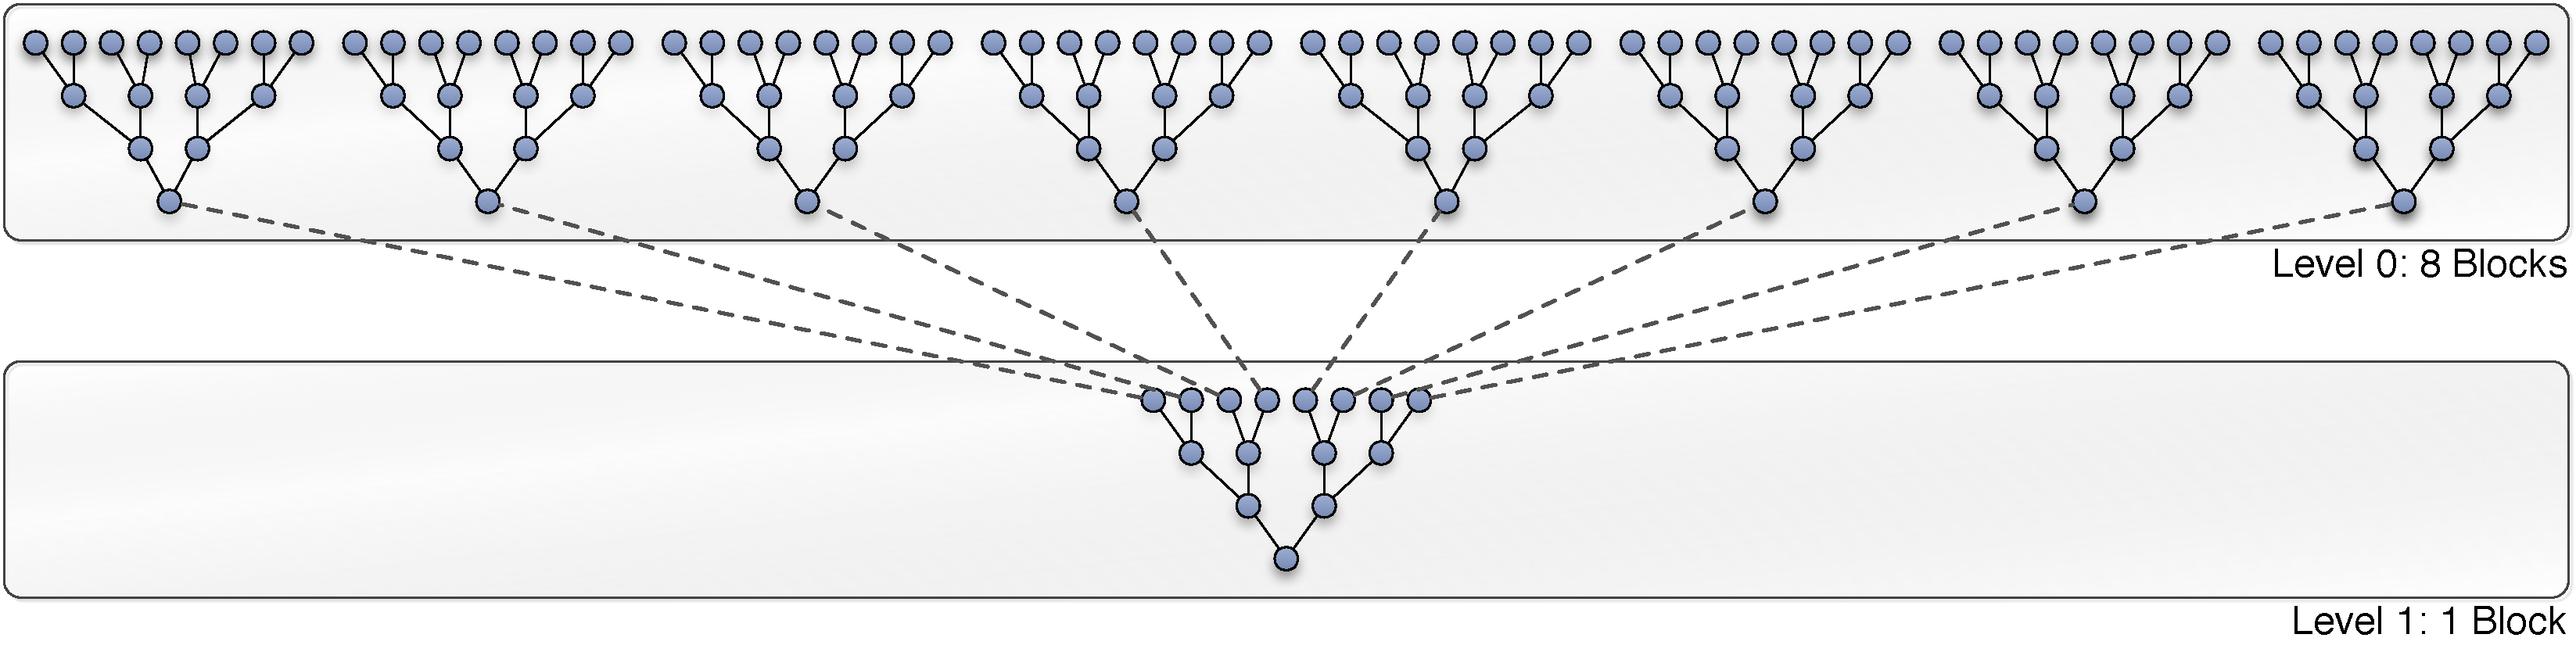
\includegraphics[width=\textwidth]{images/sec-4/tree-reduction}
    \end{center}
    \caption[A parallel tree reduction]{Illustration of a tree reduction,
        performed in two steps. In the first step 8 thread blocks in parallel
        reduce eight segments of the array to a single element each. The thread
        blocks synchronise by writing their result to memory, and the kernel is
        called recursively until the final scalar result is computed.}
    \label{fig:tree_reduction}
\end{figure}

Note that if we wish to fuse other operations into the fold kernel, only the
first line of reductions at level zero perform the fused operation. All
subsequent reductions in that kernel, as well as the recursive steps at level
one and beyond, are pure reductions. We discuss fusion further in
section~\ref{sec:array_fusion}.
% Thus, the fused operation requires compilation of two separate kernels.
% We focus on the level zero kernel, which is more interesting.

\subsubsection{Parallel Reduction Complexity}
\label{sec:parallel_reduction_complexity}

% \marginnote{tk: for non power-of-2 n, add upper/lower bounds symbols}
If each thread combines two elements at a time, then a vector of length $N$ will
be reduced in $\mathcal{O}\left( \log N \right)$ parallel steps. Each step $S$
does $\sfrac{N}{S^2}$ independent operations, so the \emph{step
complexity}\index{complexity!step} of the algorithm is:
\[
\mathcal{O}\left( \log N \right)
\]
For $N=2^{D}$, the algorithm thus performs $\sum_{S=1}^{D}2^{D-S} = N - 1$
operations. This means that the \emph{work complexity}\index{complexity!work} of
the algorithm is:
\[
\mathcal{O}\left( N \right)
\]
and so does not perform more work than a sequential algorithm. For $P$ threads
running physically in parallel on $P$ processors, the \emph{time
complexity}\index{complexity!time} is $\mathcal{O}\left( \sfrac{N}{P} + \log N
\right)$. In a thread block $N = P$, so the time complexity is:
\[
\mathcal{O}\left( \log N \right)
\]
Compare this to a sequential reduction, which has a time complexity of
$\mathcal{O}\left( N \right)$.

\subsubsection{Algorithm Cascading}
\label{sec:algorithm_cascading}

The \emph{cost} of a parallel algorithm is the number of processors $\times$
time complexity. This implies that the cost of the algorithm is
$\mathcal{O}\left( N \log N \right)$, which is \emph{not} cost efficient.

Brent's theorem~\cite{Chatterjee:2009vh} suggests that instead of each thread
summing two elements, \emph{algorithm cascading} can be used to combine a
sequential and parallel reduction. Each thread does $\mathcal{O}\left( \log N
\right)$ sequential work, which reduces the cost of the algorithm to
$\mathcal{O}\left( \sfrac{N}{\log N} \log N \right)$, or rather:
\[
\mathcal{O}\left( N \right)
\]
while keeping the work complexity $\mathcal{O}\left( N \right)$ and step
complexity $\mathcal{O}\left( \log N \right)$.

At an example, this result implies that a block of 256 threads should sum a
total of 2048 elements. In practice it is beneficial to do even more sequential
work per thread, since this reduces the number of levels in the recursive tree
reduction and provides better latency hiding.


\subsubsection{Mapping to CUDA Threads}

Reduction of a one dimensional array uses multiple thread blocks to
cooperatively reduce the array, as described above. The number of thread blocks
is limited to the maximum number of blocks that can be simultaneously resident
on the current device, which requires that blocks each do a larger amount of
sequential work before beginning the cooperative reduction phase. This limits
the total kernel startup cost associated with launching thread blocks. Since the
maximum number of resident blocks is typically much less than the number of
threads in a block, the reduction will typically require at most two kernel
invocations.\footnote{Accelerate selects the thread block size in order to
maximise thread occupancy. As this depends on both the specific GPU being used
as well as the user function the array is reduced with, an upper bound of two
parallel steps can not be guaranteed.}

Higher-dimensional reductions reduce the array along the innermost dimension
only. This is similar to a segmented fold, except that the segment descriptor is
not necessary since the length of every segment is the same and can be
determined from the array shape. Instead of thread blocks cooperatively reducing
each segment sequentially, each segment is reduced by a single thread block
which operates independently of all other thread blocks. A consequence of this
is that proper device utilisation depends on the shape of the array and not
simply the total number of elements in the array. For example, reduction of an
array with shape @(Z :. 1 :. n)@ will use a single thread block, no matter
how large @n@ is. This simplifies the implementation but is clearly not
always ideal.\footnote{The number of multiprocessors on a device various between
architecture generation and performance of a given card. For example, a Tesla
T10 processor (compute capability 1.3) has 240 cores split over 30
multiprocessors, while a Kepler K20X processor (compute capability 3.5) has 2688
cores split over only 14 multiprocessors. A given architecture generation will
have the same number of cores per multiprocessor, and lower performance
processors in a generation are produced by incorporating (or activating) fewer
multiprocessors, thereby reducing the total core count.}

A segmented reduction uses a single warp to reduce each segment. Investigation
of whether it is more efficient to implement the multidimensional reduction
using this warp-per-segment strategy, rather than mapping one thread block per
segment as is done currently, is left for future work.


\subsection{Scan}
\label{sec:parallel_scan}

Parallel scan and segmented scan algorithms are a crucial building block for a
great many data-parallel algorithms~\cite{Blelloch:1990ts,Chatterjee:1990vj}.
They also form the basis for efficiently mapping nested data-parallel languages
such as NESL~\cite{Blelloch:1995ut,Blelloch:1996jx} on to flat data-parallel
machines. Because of their fundamental importance to many algorithms,
implementing efficient scan operations in CUDA has received much
attention~\cite{Sengupta:2007tc,Sengupta:2008ut,Dotsenko:2008fo,Harris:2012fy}.

\begin{figure}
    \begin{center}
        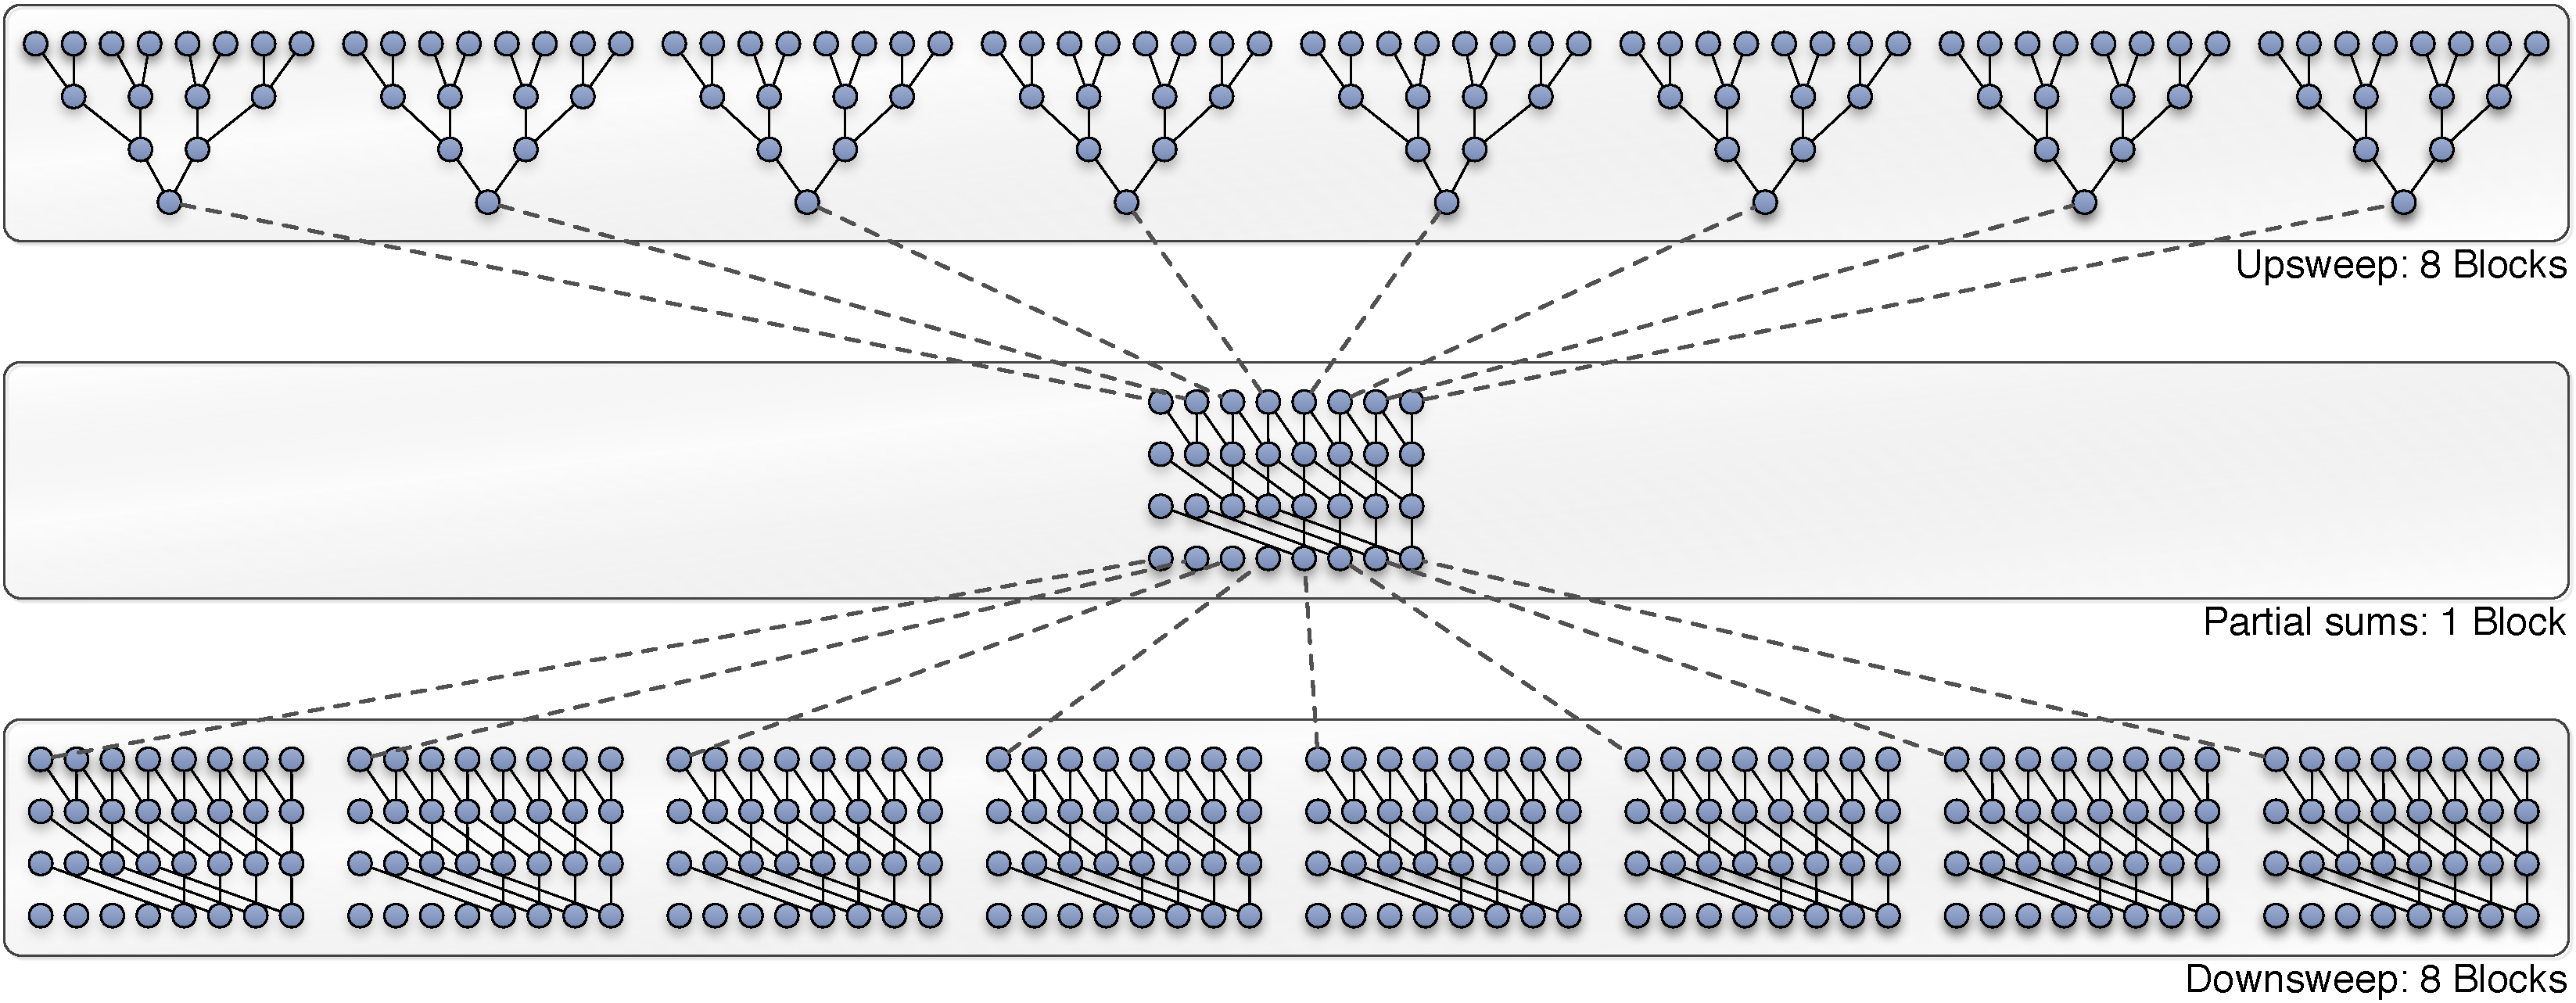
\includegraphics[width=\textwidth]{images/sec-4/scan}
    \end{center}
    \caption[A parallel inclusive scan]{Illustration of a parallel inclusive
        left-to-right scan, which is performed in three steps. In the first
        step, 8 thread blocks compute the partial scan result for each eight
        element section of the array. The partial results are then scanned by a
        single thread block in the second step. In the final phase, the 8 thread
        blocks use the partial results as the initial element when computing the
        final scan result for this section of the array.}
    \label{fig:fast_scan}
\end{figure}

The basic binary-tree based scan algorithm proceeds in $\log N$ stages.
% As shown in Figure~\ref{fig:fast_scan}, the binary operator is applied to two
% distinct elements of the input array and the output is stored into a new array.
In order to compute scans efficiently on the GPU, the input array is decomposed
into a number of blocks of size $B$, such that the scan of $B$ elements can be
computed by a thread block locally in shared memory. This inclusive scan
algorithm depicted in Figure~\ref{fig:fast_scan} proceeds in three phases:
%
\begin{enumerate}
\item All blocks are scanned in parallel, and the partial result (final scan
    value) from each block @i@ is stored into an intermediate array
    @block_results[i]@. Note that even though we require only the final value,
    because scans are directional --- either to the left or right --- we still
    compute the entire scan and return only the final value, to ensure that
    elements are processed in the correct left-to-right or right-to-left order.

\item A single thread block performs a scan of the helper array @block_results@.
    Accelerate is set up such that the number of blocks in the first step is
    less than the maximum thread block size (\S\ref{sec:executing_programs}), so
    this step does not need to repeatedly apply the global scan algorithm.

\item All blocks scan the array in parallel again, where thread block @i@ uses
    element @i@ of the result of step 2 as the initial element.

\end{enumerate}

For an exclusive scan, it is only necessary to ensure that the computation of
the partial block sums includes the seed element.


\subsubsection{Segmented scan}

Segmented scans are not implemented as primitive operations in Accelerate.
Instead, segmented scans are implemented in terms of unsegmented scans by
operator transformation~\cite{Schwartz:1980cy,Blelloch:1990ts}. Given the
operator $\oplus$ we can construct a new operator $\oplus^s$ that operators on a
flag-value pairs $\left( f_x, x \right)$ as follows:
%
\begin{equation*}
    \left( f_x, x \right) \oplus^s \left( f_y, y \right)
        = \left( f_x | f_y,\:\mathrm{if}\;f_y\;\mathrm{then}\;y\;\mathrm{else}\;x\oplus y \right)
\end{equation*}

Segmented operations often arise when dealing with nested parallelism and the
flattening transformation~\cite{Blelloch:1995ut}. In future it may be beneficial
to implement segmented scans directly rather than by operator
transformation~\cite{Sengupta:2008ut,Dotsenko:2008fo}.


\subsubsection{Interaction with array fusion}

In the scan algorithm described above, the input array to be scanned is read
twice: once when computing the partial block results, and a second time when
computing the final scanned array. If the input does not refer to manifest array
data, but instead an array in a symbolic form resulting from array fusion
(\S\ref{sec:array_fusion}), then the elements of the delayed array --- which
might contain arbitrarily expensive computations --- will be computed twice
also.

In order to avoid this, in some circumstances it might be beneficial for either
(a) the first phase of the scan to store the entire partial scan result, rather
than just the final element; or (b) to always read in manifest data, effectively
disallowing producer/consumer fusion (\S\ref{sec:array_fusion}) for
scans in the CUDA backend. The latter option is undesirable, and the former may
not work for non-commutative operators, such as the one we used in the
operator-transformation-based definition of segmented scan. It is left to future
work to fully investigate this interaction between array fusion and operations
such as scan, where the underlying implementation requires multiple passes over
the input data.

% In order to avoid this, it might seem that one approach could be for each thread
% block in the first phase to write its entire partial scan result to memory,
% which would include any computations that were part of the fused array, rather
% than just the final element. In the third phase, each block would then combine
% the partial result from the second stage to each element of the partial scan
% result from the first phase (in effect a @map@ operation). However, this would
% not correctly handle non-commutative operators, something we took advantage of
% in the definition of segmented scans.


\subsection{Permute}
\label{sec:parallel_permute}

The @permute@ collective operation defines a forward permutation $f$ as an
index mapping from one array $X$ onto the result array $Y$, which we can write
as  $f : X \rightarrow Y$. Implementation of the permute function in Accelerate
is complicated because we have not placed any particular restrictions on $f$,
namely:
%
\begin{enumerate}
    \item $f$ is not surjective: the range of $f$ may not cover the codomain
        $Y$. For every $x$ in $X$, $f\left( x \right)$ need not yield every
        index $y$ in $Y$. This means that the result array must first be
        initialised with a set of default values.

    \item $f$ is not injective: distinct elements of the domain may
        map to the same element in the codomain. For all $x$ and $x'$ in $X$, if
        $f\left( x \right) = f\left( x' \right)$, we may have that $x \ne x'$.
        This means we require an associative combination function to combine
        elements from the domain that map to the same index in the codomain.

    \item $f$ is partial: elements of the domain may be ignored, and thus do
        not map to elements in the codomain.
\end{enumerate}

That the permutation function admits partial functions in the index mapping is
not particularly challenging for the implementation, and indeed is useful for
implementing the @filter@ operation, shown in Listing~\ref{lst:filter}. The
special value @ignore@ is used to drop elements of the input vector that do not
satisfy the predicate, by not mapping those indices to an index in the codomain.
%
\begin{lstlisting}[style=haskell_float
    ,label=lst:filter
    ,caption={[Filter] Filtering returns only those elements of a
    vector which satisfy a predicate. This operation is included as part of
    Accelerate's standard prelude.}]
filter :: Elt a => (Exp a -> Exp Bool) -> Acc (Vector a) -> Acc (Vector a)
filter p vec
  = let flags            = map (boolToInt . p) vec
        (targetIdx, len) = scanl' (+) 0 flags
        defaults         = backpermute (index1 $ the len) id vec
    in
    permute const defaults (\ix -> flags!ix ==* 0 ? (ignore, index1 $ targetIdx!ix)) vec
\end{lstlisting}

On the other hand, because we can not prove that @filter@ is surjective, we
require the result vector to be first initialised with default values. Since we
do not know anything about the element type @a@, the only recourse is to
copy elements from the input array @vec@. This is doubly wasteful, because
we must first execute the @backpermute@ kernel to compute the
@defaults@ array, and then copy those values into the results vector before
executing the @permute@ kernel, even though we know the initialised values
will be completely overwritten.

At a second example, Listing~\ref{lst:histogram} demonstrates the computation of
a simple ten bin histogram from a vector of floating point elements in the range
$\left[ 0, 100 \right)$. In this case the permutation function is neither
surjective nor injective, as some bins may contain no elements and thus take the
default value, while other bins may contain multiple elements which need to be
combined (accumulated) correctly.
%
\begin{lstlisting}[style=haskell_float
    ,label=lst:histogram
    ,caption={[Simple histogram] A simple histogram written in
    Accelerate. We assume the input vector contains elements in the range
    $\left[0,100\right)$ and accumulate into ten equally sized bins.}]
histogram :: Acc (Vector Float) -> Acc (Vector Int)
histogram vec
  = let bins      = 10
        zeros     = fill (constant (Z :. bins)) 0
        ones      = fill (shape vec)            1
    in
    permute (+) zeros (\ix -> index1 (A.floor ((vec ! ix) / P.fromIntegral bins))) ones
\end{lstlisting}

The semantics of the operation is that every permutation from source to result
array is applied at the same time in a single parallel step. If multiple CUDA
threads attempt a non-atomic write to the same memory location at the same time,
the writes will be serialised but the thread which performs the final write is
undefined, and so the final value at that memory slot is also
undefined~\cite{NVIDIA:2012wf}. To support non-injective permutation functions,
which are required to evaluate the histogram program correctly, the atomic
compare-and-swap operation is used to implement write combining.\footnote{The
atomic compare-and-swap operation on 32-bit values into global memory is only
available for devices of compute capability 1.1 and higher, and for 64-bit
values on devices of compute capability 1.2 and higher.} For a combination
function @f@ on elements of type @T@, the following atomically combines a value
from the source array @x@ with the value of the result array @y@:

\begin{lstlisting}[style=cuda]
  T x        = source[i];
  T y, old_y = result[j];
  do {
      y     = old_y;
      old_y = atomicCAS(&result[j], y, f x y);
  } while (y != old_y);
\end{lstlisting}
%
Any atomic operation on simple types can be implemented in terms of
compare-and-swap in this manner. Utilising more specific atomic operations such
as @atomicAdd@ when available is left to future work.


\subsubsection{Implementation using explicit locking}

The implementation for combining elements of the permutation function works well
for simple atomic types, but as Accelerate uses a struct-of-arrays
representation (\S\ref{sec:representing_tuples}, combining tuple types must
apply the procedure to each component of the tuple separately, which can lead to
inconsistencies.\footnote{\url{https://github.com/AccelerateHS/accelerate/issues/137}}

One alternative would be to explicitly lock each element of the output array
before threads can access it, and then for each thread to commit all components
of the array as a single atomic operation. A straightforward to implement this
is via a \emph{spin lock}, where threads trying to acquire the lock simply wait
in a loop (``spin''), repeatedly checking whether the lock is available. Since
the thread remains active but is not performing any useful work, the use of this
kind of busy waiting is inefficient if threads are blocked for an extended
period of time (because the lock is contended by many threads, or the atomic
section executed while the lock is held is lengthy).

Implementing a spin-lock can be done similarly to the following:
%
\begin{lstlisting}[style=cuda]
  do {
      old = atomicExch(&lock[i], 1);                                               // (1)
  while (old == 1);                                                                // (2)
    /* atomic section */                                                           // (3)
  atomicExch(&lock[i], 0);                                                         // (4)
\end{lstlisting}
%
\begin{enumerate}
    \item The spin lock procedure requires a temporary array to represent the
        lock state for each element of the output array. We use 1 to represent
        the locked state, and 0 to indicate the element is unlocked. To lock
        element @i@ of the output array, we atomically store 1 into the @lock@
        slot for this element, returning the @old@ state of the lock.

    \item If the @old@ state of the lock was unlocked (0) then we just acquired
        the lock. Otherwise it was already locked, so we must retry.

    \item Once the lock is acquired, the atomic section can be computed.

    \item To release the lock, write zero back into the lock slot for this
        element. A memory barrier or atomic operation, as used here, is required
        for this step to ensure memory consistency on architectures which do not
        have a strong memory model, such as CUDA devices.
        % (later x86 architectures can safely use an unlocked @MOV@ instruction).

\end{enumerate}

It is left to future work to fully investigate the use of spin locking as an
alternative strategy for combining elements in the permute operation.


\subsection{Stencil}
\label{sec:parallel_stencil}

Stencil operations are a fundamental building block of many scientific and image
processing algorithms. A stencil computation is similar to a @map@, that has
access to the elements in the local neighbourhood surrounding the element. For
example, at the core of many image processing algorithms is the convolution
operator $*$, whose definition is as follows:

\begin{equation*}
    (A * K)(x, y) = \sum_i \sum_j A(x+i, y+j) K(i,j)
\end{equation*}
%
Here $A$ is the image being processed and $K$ is the \emph{convolution kernel}
or \emph{stencil}. A \emph{stencil} is a small matrix that defines a
transformation on the image. Typical transformations include Gaussian blur and
the Sobel differentiation operator, both of which are used in the Canny edge
detection algorithm (\S\ref{sec:canny}).


\subsubsection{Bounds checking}

Since the stencil has access to elements in the surrounding neighbourhood, an
immediate concern is what to do when the stencil ``falls off'' the edge of the
array. Figure~\ref{fig:stencil3x3} shows the application of a $3\times3$ stencil
in this circumstance. The white squares indicate the \emph{internal} region
where the stencil is entirely within the array, and the grey squares indicate
the \emph{border} region, where part of the stencil falls lies outside of the
array boundary.

\begin{figure}[tbp]
    \begin{center}
        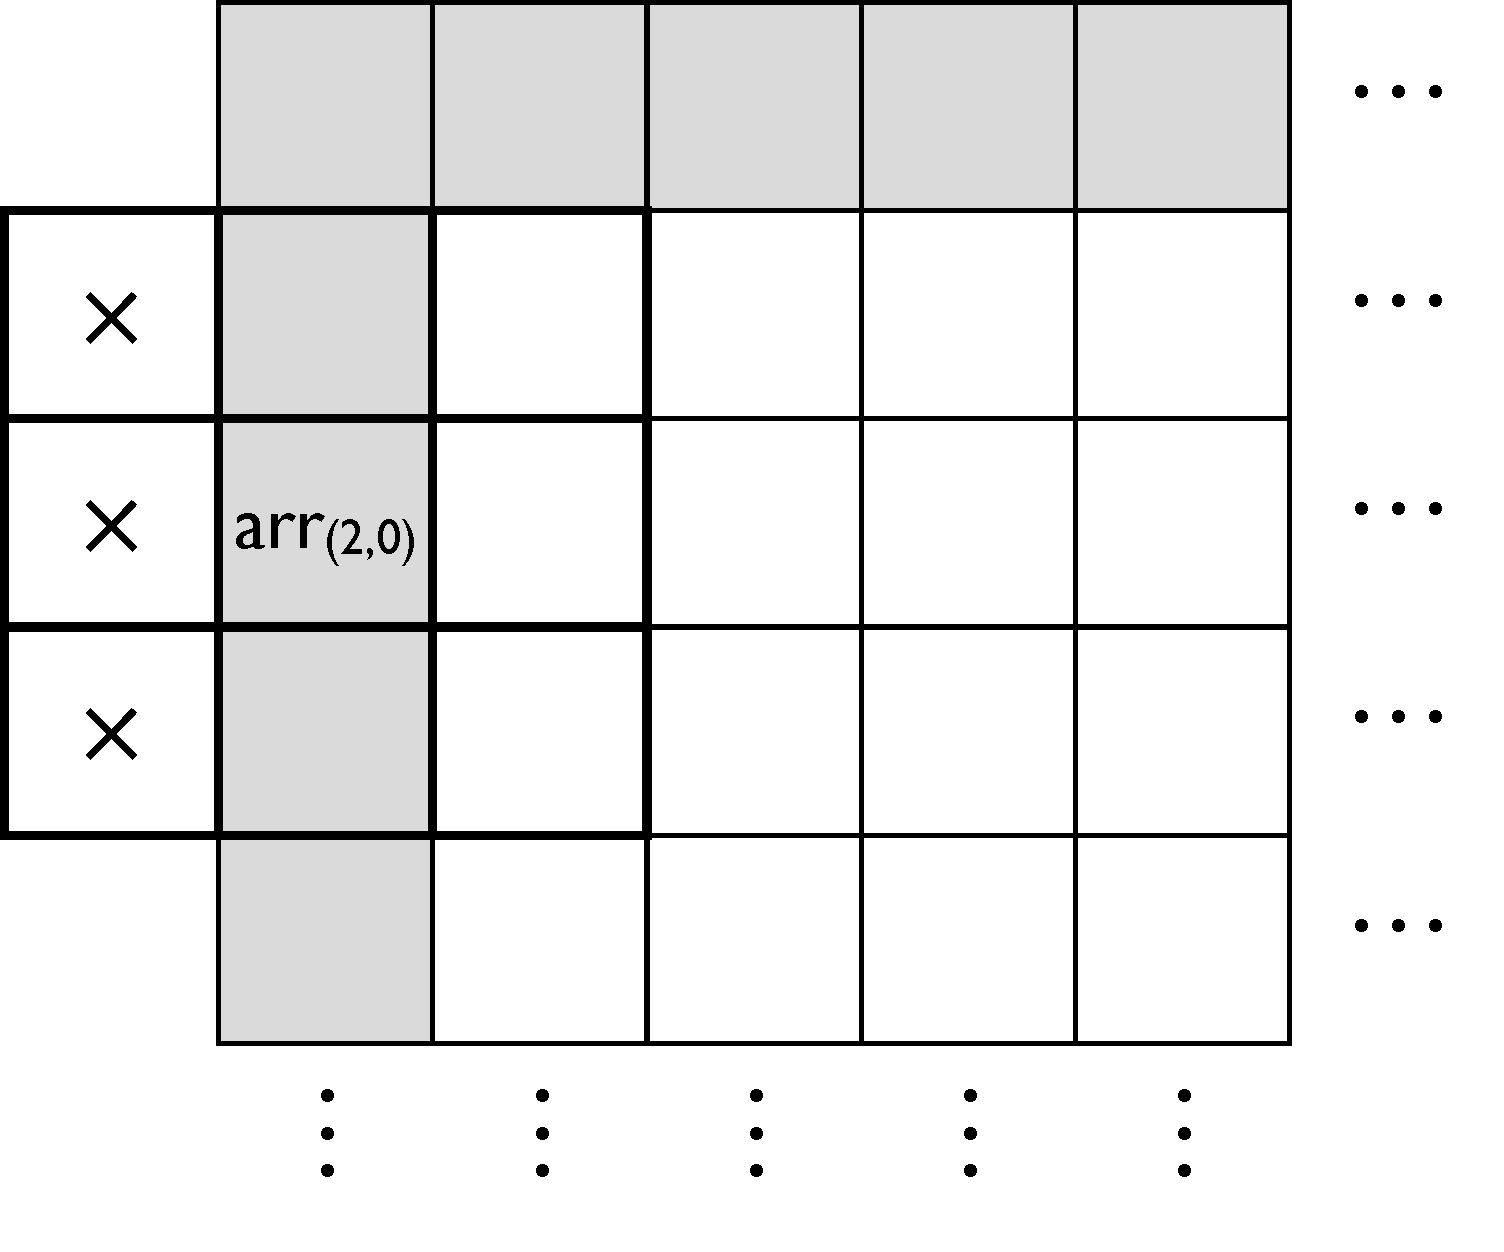
\includegraphics[width=0.5\textwidth]{images/sec-4/stencil3x3}
    \end{center}
    \caption[Application of a $3\times3$ stencil in the border region]
        {Application of a $3\times3$ stencil in the border region. Elements in
        the border region (grey), such as the indicated element at index
        \code{(Z:.2:.0)}, have neighbouring elements which might fall outside
        the array bounds, whereas for elements in the internal region (white)
        the stencil lies entirely within the array.}
    \label{fig:stencil3x3}
\end{figure}

Boundary conditions determine how to handle out-of-bounds neighbours, by
specifying a constant value to use instead, or by reading the source array at a
different index. However, with the array sizes typical of GPU programs, the
border region represents only a tiny fraction of the entire array. For example,
a 512-pixel square image has less than one percent of its pixels along the edge.
This fact implies that for optimal performance, we should avoid testing of the
boundary each time we read an element from the source array. For simple
convolutions such as those used by Canny (\S\ref{sec:canny}), this adds
significant overhead~\cite{Lippmeier:2011cd}. Separating computation of the
border and internal region is left for future work.


\subsubsection{Overlapping elements}

Suppose we wish to apply a dense $3\times3$ stencil to a single internal point
in the array, where each element of the stencil is utilised. Application of the
stencil requires at least nine elements of the array to be loaded, and one store
for the result.

\begin{figure}[tbp]
    \begin{center}
        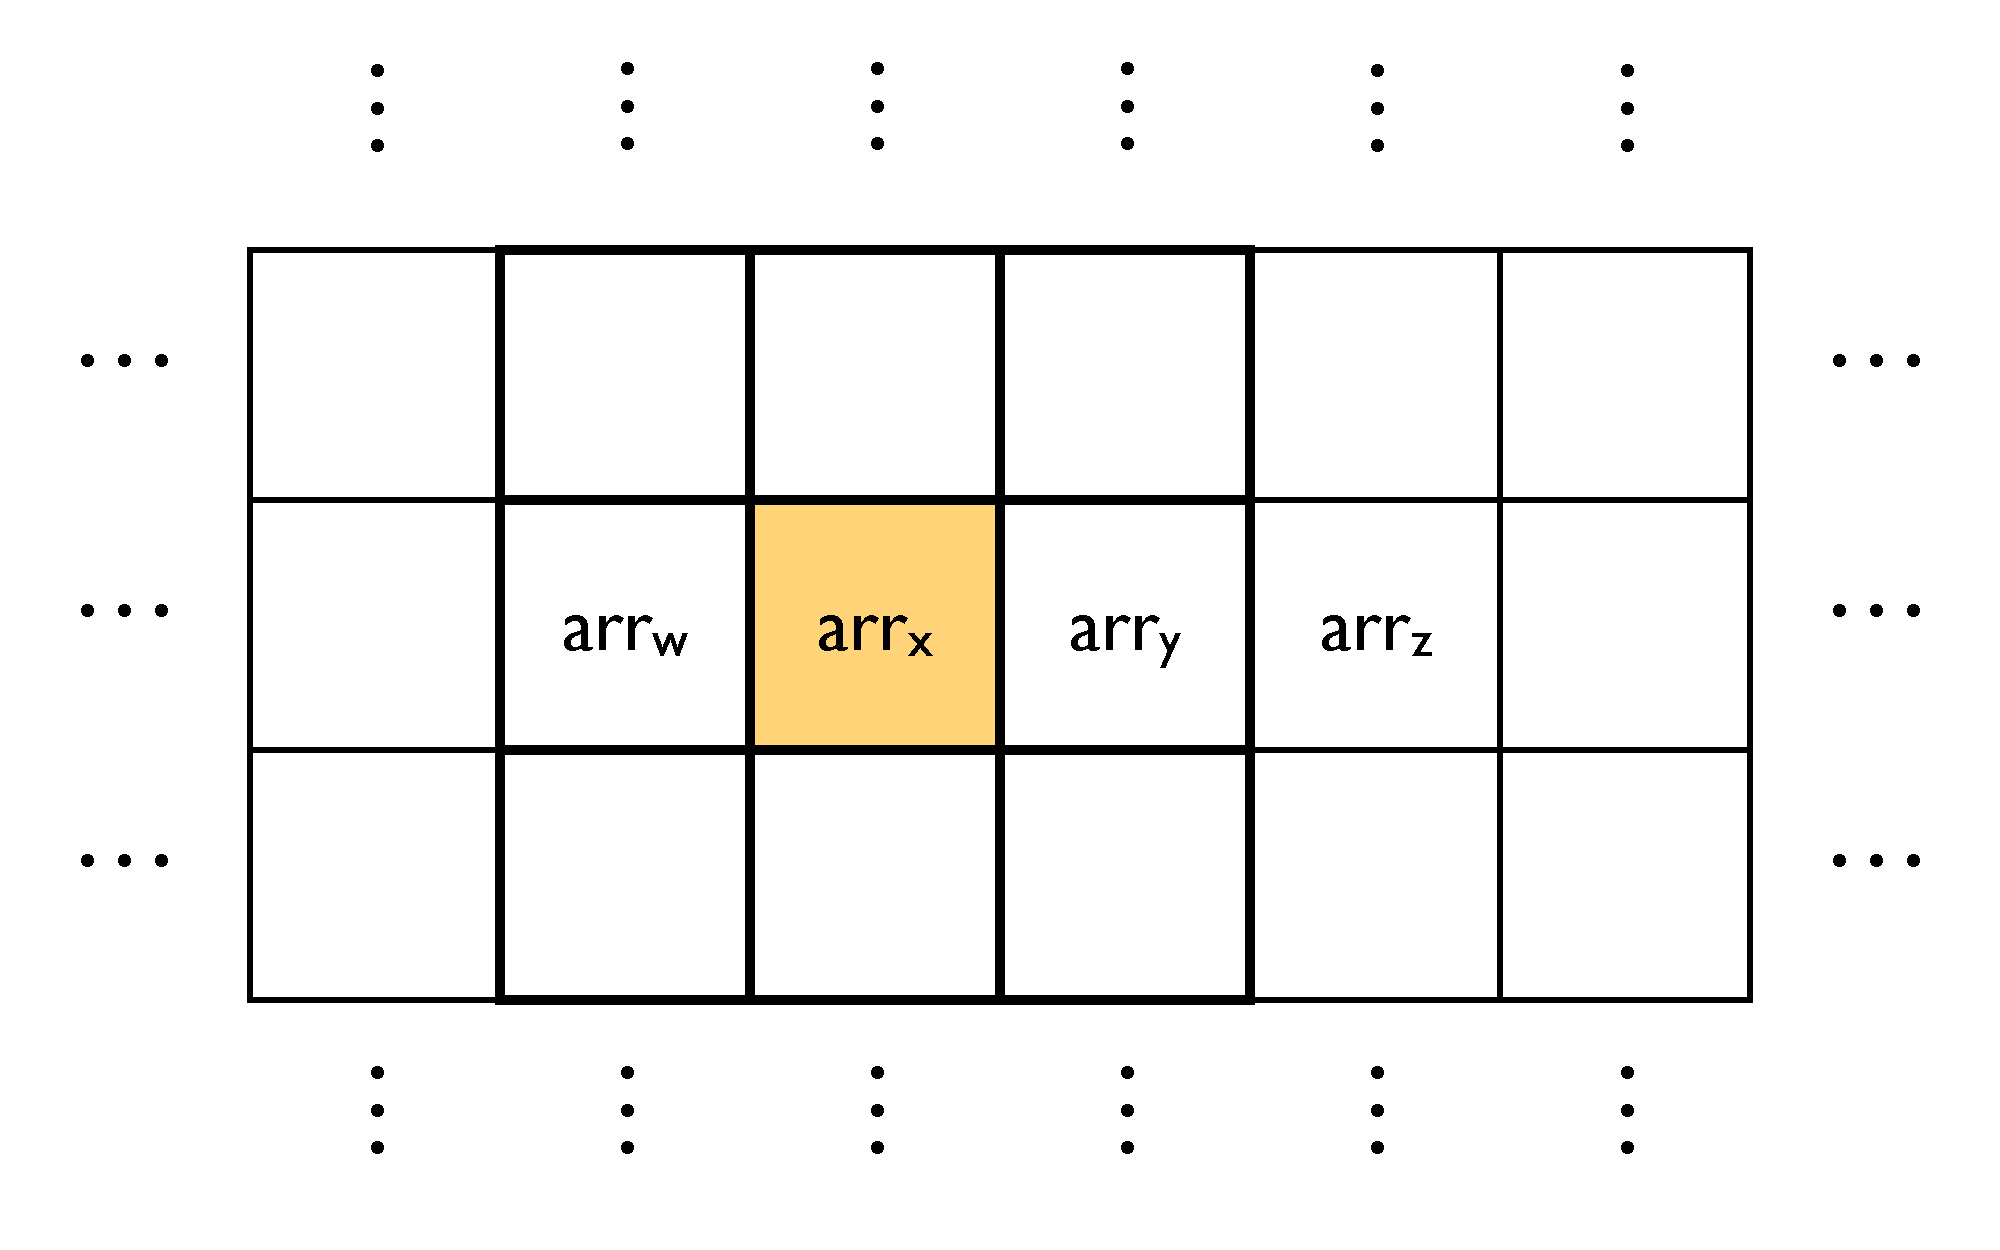
\includegraphics[width=0.6\textwidth]{images/sec-4/stencil-sharing}
    \end{center}
    \caption[Overlapping elements in a $3\times3$ stencil]{
        Overlapping elements in a dense $3\times3$ stencil. Computation of each
        element requires nine reads from the source array. If the four elements
        cooperate to share the source data, the number of loads to the source
        array is halved.}
    \label{fig:stencil_sharing}
\end{figure}

Figure~\ref{fig:stencil_sharing} shows the evaluation of four horizontally
adjacent elements. If we evaluate these points independently, we would need
$4 \times 9 = 36$ loads of the source array, plus the four stores to the result
array. However, if the calculation of these four elements can cooperate and
share loads from the source array into a local temporary array, this would
requires only $3 \times 6 = 18$ loads, plus the four stores. Sharing of stencil
elements can thus significantly reduce memory bandwidth requirements.

Sharing of stencil elements in CUDA can be achieved by having the thread block
first cooperatively read the stencil elements into \indexe{shared
memory}~\cite{NVIDIA:2012wf}, and then each thread computes its stencil function
using these shared values. In Accelerate, sharing of stencil elements is
complicated by two main factors:
%
\begin{enumerate}
    \item Stencil patterns can be large: up to 9 elements in each dimension.
        Since the shared memory region on the GPU is usually very small, this
        can significantly limit the maximum thread block size. If the occupancy
        of the device is too low, there may be insufficient parallelism to hide
        global memory transfer latency.

    \item A stencil function does not need to use all elements defined in the
        pattern, so reading all elements into shared memory could waste more
        bandwidth than it saves. The pattern also does not need to be square nor
        symmetric, which complicates efficient cooperative loading of the
        common elements into shared memory.
\end{enumerate}

The implementation currently ignores this issue and does not explicitly share
elements between threads, instead relying on the cache. For older (compute 1.x)
devices that lack a traditional cache mechanism to global memory, we read the
source array using the texture cache.\footnote{A holdover from the graphical
heritage of the GPU.} It is left to future work to implement sharing of stencil
elements between threads, either in general or specialised for certain cases
such as dense stencils or those commonly used for convolutions.


\subsubsection{Interaction with array fusion}

Since the stencil operation has access to the elements surrounding the focal
point of the stencil, if the input is represented by a symbolic array resulting
from array fusion (\S\ref{sec:array_fusion}), rather than manifest array data,
accessing these neighbouring elements implies recomputing the symbolic
computations on every element access. For some operation @stencil s . map f@, if
the results of @f@ can be shared between threads of the stencil (previous
section), or if @f@ is cheap, then the duplicate computations required to fuse
the two operations might be preferable to the extra memory bandwidth required to
store the result of @map f@ to memory. A full exploration of stencil-aware array
fusion is left to future work.


\section{Manipulating embedded programs}
\label{sec:manipulating_embedded_programs}

The Accelerate core language is richly typed, maintaining full type information
of the embedded language in the term tree. In order to apply transformations to
these terms while maintaining the correctness of the program as encoded in its
type, we require methods to manipulate these richly typed terms in a type- and
scope-preserving manner. This section covers several technique for manipulating
the embedded Accelerate programs, that are required to implement the
optimisations discussed in the following chapter.


\subsection{Typed equality}
\label{sec:equality}

If we want to test whether two Accelerate terms are equal --- for example, to
determine whether the subexpressions can be shared --- we immediately run into
the problem that terms in the core Accelerate language are existentially typed.
That is, how should we implement:
%
\begin{lstlisting}[style=haskell]
Exp s == Exp t = ??
\end{lstlisting}
%
There is no reason that @s@ and @t@ should be expressions of the same
type. In some instances we might not care, and as such can define standard
heterogeneous equality:
%
\begin{lstlisting}[style=haskell]
instance Eq (PreOpenExp acc env aenv t) where
    (==) = heq
    where heq :: PreOpenExp acc env aenv a -> PreOpenExp acc env aenv b -> Bool
          heq = ...
\end{lstlisting}
%
where we do not care about the result type of each expression, and only require
that the environment type, re size, of free scalar and array variables are the
same so that we can test equality of \indext{de Bruijn} indices.

However, we often \emph{do} care about the specific types of our existentially
quantified terms. Consider the case of defining equality for let-bindings.
The Accelerate scalar language defines let-bindings of the embedded program as a
constructor of a GADT~\cite{Jones:2006eh}, whose type tracks the type and scope
of the bound term (\S\ref{sec:richly_typed_terms}):
%
\begin{lstlisting}[style=haskell]
data PreOpenExp acc env aenv t where
    Let :: (Elt bnd_t, Elt body_t)                      -- Local binding of a scalar expression
        => PreOpenExp acc env          aenv bnd_t       -- bound term
        -> PreOpenExp acc (env, bnd_t) aenv body_t      -- body/scope of binding
        -> PreOpenExp acc env          aenv body_t

    -- other language constructs\ldots
\end{lstlisting}
%
To apply @heq@ to the body expression, we need to know something about
the type of the bound terms to ensure that the scalar environments are the same,
namely \lstinline[style=inline,mathescape]{a $\sim$ bnd_t $\sim$ b}.%
\footnote{Alternatively we can use \footcode{Data.Typeable.gcast} to provide a
type-safe cast, but this quickly becomes unwieldy and is a little
unsatisfactory.} To do this we must equip terms with a runtime witness to the
existentially quantified type. Our reified dictionaries will allow us to do
exactly this, so we can define heterogeneous equality for reified dictionaries:
%
\begin{lstlisting}[style=haskell]
heqIntegralType :: IntegralType s -> IntegralType t -> Bool
heqIntegralType (TypeInt _)  (TypeInt _)  = True
heqIntegralType (TypeWord _) (TypeWord _) = True
  ...
heqIntegralType _            _            = False
\end{lstlisting}
%
However, doing this is perfectly useless as it only gives us a value of type
@Bool@, with no idea what that value means or to what its truth might
entitle us. The type checker does not gain any useful knowledge about the types
the dictionaries @a@ and @b@ witness simply by knowing that
@heqIntegralType a b = True@. A boolean is a bit uninformative.

Instead, we can write essentially the same test, but in the positive case
deliver some \emph{evidence} that the types are equal:
%
\begin{lstlisting}[style=haskell]
data s :=: t where
    REFL :: s :=: s

matchIntegralType :: IntegralType s -> IntegralType t -> Maybe (s :=: t)
matchIntegralType (TypeInt _)  (TypeInt _)  = Just REFL
matchIntegralType (TypeWord _) (TypeWord _) = Just REFL
  ...
matchIntegralType _            _            = Nothing
\end{lstlisting}
%
Matching on @Just REFL@ will inject the knowledge into the type
checker that the types @s@ and @t@ are the same. Now with our
evidence-producing heterogeneous equality test for reified dictionary families,
we can compare two terms and gain type-level knowledge when they witness the
same value-level types. These witnesses for existentially quantified types then
allow us to test for equality \emph{homogeneously}, ensuring that positive
results from singleton tests give the bonus of unifying types for other tests:
%
\begin{lstlisting}[style=haskell]
matchPreOpenExp
    :: PreOpenExp acc env aenv s
    -> PreOpenExp acc env aenv t
    -> Maybe (s :=: t)
matchPreOpenExp (Let x1 e1) (Let x2 e2)
  | Just REFL <- matchOpenExp x1 x2     -- if the bound expressions match
  , Just REFL <- matchOpenExp e1 e2     -- then the environment of the body term will also match
  = Just REFL

matchPreOpenExp ...
\end{lstlisting}


\subsubsection{Congruence}

As we are interested in the facility of matching terms for the purposes of
optimisations such as common subexpression elimination (\S\ref{sec:cse}), it is
beneficial to define not equality but instead \indexe{congruence} of terms. Two
nodes are considered congruent if the nodes they label are constants and the
constants are equal; or they have the same operator and the operands are
congruent. The crux of the latter condition refers to commutative relations,
such as scalar addition, where an operator yields the same result when the order
of the operands are reversed. When checking equality of primitive applications,
we discriminate binary functions whose arguments commute, and return those
arguments in a stable ordering by comparing a hash of each of the sub-terms.
%
\begin{lstlisting}[style=haskell]
commutes
    :: PrimFun (a -> r)
    -> PreOpenExp acc env aenv a
    -> Maybe (PreOpenExp acc env aenv a)
commutes f x = case f of
  PrimAdd _     -> Just (swizzle x)
    ...         -> Nothing
  where
    swizzle :: PreOpenExp acc env aenv (a,a) -> PreOpenExp acc env aenv (a,a)
    swizzle exp
      | Tuple (NilTup `SnocTup` a `SnocTup` b) <- exp
      , hashPreOpenExp a > hashPreOpenExp b     = Tuple (NilTup `SnocTup` b `SnocTup` a)
      | otherwise                               = exp
\end{lstlisting}


\subsection{Simultaneous substitution}
\label{sec:substitution}

In order to do things like renaming and substitution we require a value-level
substitution algorithm for the richly typed terms. The implementation follows
the method of \citet{McBride:2006up,McBride:2005jv}, where it is seen that
renaming and substitution are both instances of a \emph{single} traversal
operation, pushing functions from variables to ``stuff'' through terms, for a
suitable notion of stuff.
%
The trick is to push a \emph{type-preserving} but \emph{environment changing}
operation structurally through terms:
%
\begin{lstlisting}[style=haskell]
v :: forall t'. Idx env t' -> f env' t'
\end{lstlisting}

Where the operation differs is in the image of variables: renaming maps
variables to variables and substitution maps variables to terms. We then lift
this to an operation which traverses terms, with appropriate lifting to push
under a lambda, and rebuilding the term after applying @v@ to the
variables:
%
\begin{lstlisting}[style=haskell]
rebuild :: Syntactic f
        => (forall t'. Idx env t' -> f env' t')
        -> Term env  t
        -> Term env' t
\end{lstlisting}

The @Syntactic@ class\footnote{Since Accelerate is a stratified language
there are separate implementations of this toolkit on syntactic elements for the
scalar and collective operations, but the details are identical. The discussion
uses the generic \footcode{Term} to mean either of these operations.} tells us
everything we need to know about @f@ --- our notion of ``stuff'' --- in
order to rebuild terms: a mapping in from variables, a mapping out to terms, and
a weakening map which extends the context. Renaming will instantiate @f@
with @Idx@, whereas for substitutions we may choose @Term@ instead.
%
\begin{lstlisting}[style=haskell]
class Syntactic f where
    varIn   :: Idx env t -> f env t             -- variables embed in f
    termOut :: f env t   -> Term env t          -- f embeds in terms
    weaken  :: f env t   -> f (env, s) t        -- f allows weakening

instance Syntactic Idx
instance Syntactic Term
\end{lstlisting}

A key component of this toolkit, \indexe{weakening} describes an operation we
usually take for granted: every time we learn a new word, old sentences still
make sense; if a conclusion is justified by a hypothesis, it is still justified
if we add more hypotheses; a term remains in scope if we bind new (fresh)
variables. Weakening is the process of shifting things from one scope to a
larger scope in which new things have become meaningful, but no old things have
vanished. When we use a named representation (or HOAS\index{higher-order
abstract syntax}\index{HOAS|see{higher-order abstract syntax}}) we get weakening
for free, but in the de Bruijn\index{de Bruijn} representation weakening takes
work: we need to shift all the variable references to make room for new
bindings. To do this we need to explain how to shift the @v@ operation into
an extended environment; saying what to do with the new variable and how to
account for it on the output side.
%
\begin{lstlisting}[style=haskell]
shift :: Syntactic f
      => (forall t'. Idx env t' -> f env' t')
      -> Idx (env,  s) t
      -> f   (env', s) t
\end{lstlisting}
%
Overall, the crucial functionality of simultaneous substitution is to propagate
a class of operations on variables closed under shifting, which is what
@Syntactic@ and @rebuild@ offer.


\subsection{Inlining}
\label{sec:inlining}

\begin{lstlisting}[style=haskell_float
    ,label=lst:inlining
    ,caption={A simultaneous substitution to inline terms}]
subTop :: Term env s -> Idx (env, s) t -> Term env t
subTop s ZeroIdx      = s
subTop _ (SuccIdx ix) = Var ix

inline :: Term (env, s) t -> Term env s -> Term env t
inline body bnd = rebuild (subTop bnd) body
\end{lstlisting}

The final question, then, is how to write the function @v@ which we push
through terms, as the type @forall t'@ could be anything. After all, what
is the point of having a simultaneous substitution algorithm if we can't
specialise it to one-at-a-time substitution.

The function @subTop@ in Listing~\ref{lst:inlining} takes a replacement for the
top variable and returns a simultaneous substitution which eliminates @ZeroIdx@.
If we have a term with one free variable, we can use this to replace that
variable with a term. That is, @inline@ a term into all use sites of the free
variable.

The demonic $\forall$ --- which is to say that the quantifier is in a position
which gives us obligation, not opportunity --- of the operator @v@ forces
us to respect type: when pattern matching detects the variable we care about,
happily we discover that it has the type we must respect. The demon is not so
free to mess with us as one might at first fear.

% Typing rules; each rule types the general usage of a symbol, below the
% line, in terms of the parameters above the line.??

\subsection{Function composition}
\label{sec:function_composition}

The equivalent of unary function composition @(.)@ on terms can be
defined in a similar manner. A function @(a -> b)@ is equivalent to a
@Term@ of type @b@ and free variable @a@. Similar to inlining, we
replace an expression that uses the top variable with one that uses another,
remembering to bind the result of the first expression so that it can be reused
in the second without duplication.

\begin{lstlisting}[style=haskell_float
    ,label=lst:function_composition
    ,caption={A simultaneous substitution to compose unary function terms}]
dot :: Term (env, b) c -> Term (env, a) b -> Term (env, a) c
dot f g = Let g (rebuild split f)
  where
    split :: Idx (env, b) c -> Term ((env, a), b) c
    split ZeroIdx      = Var ZeroIdx
    split (SuccIdx ix) = Var (SuccIdx (SuccIdx ix))

compose :: Fun env (b -> c) -> Fun env (a -> b) -> Fun env (a -> c)
compose (Lam (Body f)) (Lam (Body g)) = Lam (Body (f `dot` g))
compose _              _              = error "compose: impossible case"
\end{lstlisting}

Note the type of @split@ in Listing~\ref{lst:function_composition}, which
creates space in the environment at the second index (@SuccIdx ZeroIdx@) for the
free variable @a@ to appear in the resultant @Term@, as the first index will be
bound to the result of the first expression @g@.

The function @compose@ finally lifts this to function terms by unwrapping the
lambda abstractions. Annoyingly, GHC's type checker can not determine that the
function type prohibits any valid term except those with a single lambda, so we
need a second catch-all case to suppress a compilation warning. In the remainder
of the text, we elide the impossible cases for brevity.


\subsection{Environment manipulation}
\label{sec:environment_manipulation}

As part of the fusion transformation of recasting terms we often need to lift
array valued inputs to be let-bound at higher points to avoid work duplication,
but at the same time we can not immediately add these bindings to the output
term because they will interfere with further fusion steps. We need to collect
these extra bindings separately from the main term, and add them to the output
term at some later point. Furthermore, we must ensure we correctly track the
types of the environments between the fused terms and the collected
let-bindings.

Listing~\ref{lst:Extend} defines a heterogeneous snoc-list of array terms that
witnesses how an array environment is extended by the application of these
operations.
%
\begin{lstlisting}[
    style=haskell_float,
    label={lst:Extend},
    caption={Extending an array environment}]
data Extend acc aenv aenv' where
    BaseEnv :: Extend acc aenv aenv
    PushEnv :: Arrays a
            => Extend     acc aenv aenv'
            -> PreOpenAcc acc      aenv' a
            -> Extend     acc aenv (aenv', a)
\end{lstlisting}
%
In the style of the \indext{de Bruijn} indices used for projecting environment
variables (\S\ref{sec:richly_typed_terms}), @Extend@ uses an inductive notion of
tuples as heterogeneous \emph{snoc} lists. In contrast to environment indices,
the base case does not refer to an empty environment, but instead the
environment @aenv@ which we are extending. This witnesses how to construct an
extended environment @aenv'@ by bringing new terms into scope, one at a time.
%
\begin{lstlisting}[style=haskell]
bind :: Arrays a
     => Extend     acc aenv aenv'
     -> PreOpenAcc acc      aenv' a
     -> PreOpenAcc acc aenv       a
bind BaseEnv         = id
bind (PushEnv env a) = bind env . Alet (inject a) . inject
\end{lstlisting}
%
The auxiliary function @inject :: PreOpenAcc acc aenv a -> acc aenv a@ completes
the knot tying trick (\S\ref{sec:knot_tying}) to complete the definition of each
of the array terms.


\subsubsection{Sinking}
\label{sec:sinking}

\begin{lstlisting}[
    style=haskell_float,
    label=lst:sinking,
    caption={Sinking terms to a larger environment}]
type env :> env' = forall t'. Idx env t' -> Idx env' t'

class Sink f where
    weaken :: env :> env' -> f env t -> f env' t

sink :: Sink f => Extend acc env env' -> f env t -> f env' t
sink env = weaken (k env)
  where
    k :: Extend acc env env' -> Idx env t -> Idx env' t
    k BaseEnv       = id
    k (PushEnv e _) = SuccIdx . k e
\end{lstlisting}

We define \emph{sinking} as the operation of shifting a term from one (array)
environment into another, where new things have come into scope according to
some witness, and no old things have disappeared.

Listing~\ref{lst:sinking} generalises @weaken@ from
section~\ref{sec:substitution} to increase the environment of an object @f@
based on some function on indices rather than shifting by a single de Bruijn
index. Thus we only need to traverse a term once no matter how many positions
the variable indices shift by. Using @sink@, we can weaken terms based on the
witness provided by @Extend@.


\section{Embedding GPU programs as skeletons}
\label{sec:code_generation}

Accelerate offers a range of aggregate operations on multi-dimensional arrays.
They include operations modelled after Haskell's list library, such as
@map@ and @fold@, but also array-oriented operations, such as
@permute@ and stencil convolutions.

As a simple example, consider the dot product of two vectors:
%
\begin{lstlisting}[style=haskell]
dotp :: Acc (Vector Float) -> Acc (Vector Float) -> Acc (Scalar Float)
dotp xs ys = fold (+) 0 (zipWith (*) xs ys)
\end{lstlisting}
%
The crucial difference to vanilla Haskell is the @Acc@ type constructor
representing \emph{embedded array-valued computations}. The types
@Vector e@ and @Scalar e@ represent one-dimensional and
zero-dimensional (singleton) arrays, respectively.

The expression @zipwith (*) xs ys@ implements point-wise multiplication of
the two argument vectors, and @fold (+) 0@ sums the resulting products up
to yield the final, scalar result, wrapped into a singleton array. The type of
@fold@ is:
%
\begin{lstlisting}[style=haskell]
fold :: (Shape sh, Elt a)
     => (Exp a -> Exp a -> Exp a)
     -> Exp a
     -> Acc (Array (sh:.Int) a)
     -> Acc (Array sh a)
\end{lstlisting}
%
It uses a binary folding function operating on \emph{embedded scalar
computations} of type @Exp a@ to implement a parallel reduction along the
innermost dimension of an $n$-dimensional, embedded array of type \code{Array
(sh:.Int) a}. The \emph{shape} @sh:.Int@ consist of a polymorphic shape
@sh@ with one added (innermost) dimension, which is missing from the shape
of the result array.


\subsection{Array operations as skeletons}

The Accelerate CUDA backend is based on the idea of \emph{algorithmic
skeletons}~\cite{Cole:1989vr}, where a parallel program is composed from one or
more parameterised skeletons, or templates, encapsulating specific parallel
behaviour. In our case, the backend implements each of the aggregate array
operations, such as @map@, by way of a CUDA C \emph{code template} that is
parameterised with array types and worker functions, such as the function to be
mapped, to be injected at predefined points.

This generative approach is attractive for specialised hardware, such as GPUs,
as the code templates can be hand-tuned to avoid expensive control flow, ensure
efficient global-memory access, and use fast on-chip shared memory for local
communication --- all of which is necessary to ensure good performance on the
GPU~\cite{NVIDIA:2012wf}.

In the first version of Accelerate, we implemented CUDA C code templates and
template instantiation with a mixture of C++ templates and C preprocessor
macros, which was described in \cite{Chakravarty:2011fr}. While workable, this
approach turned out to have a number of problems:

\begin{itemize}
    \item The use of CPP is fragile and difficult to maintain. Template
        instantiation by inlining of CPP macros required the use of fixed
        variables with no static checking to ensure the consistent use of names
        or that used names where defined before their use. Moreover it was easy
        to generate code that wasn't even syntactically valid.

    \item The approach led to the generation of dead code whenever specific
        template instances did not use all of their parameters or fields of
        structured data, which the CUDA compiler was unable to remove as dead
        code.

    \item Most importantly, the use of CPP did not scale to support the
        implementation of producer-consumer skeleton fusion, which is a crucial
        optimisation, even for code as simple as dot product.

\end{itemize}

The next sections discuss the new approach to template instantiation that avoids
these problems, and appeared in \cite{CliftonEverest:2014vi}.


\subsection{Algorithmic skeletons as template meta programs}

The code generator includes CUDA code skeletons implementing each of the
collective operations in Accelerate. Each skeleton encodes the behaviour for
each thread for this collective operation, fixing the parallel algorithmic
structure of the operation. Each skeleton contains placeholders for the inputs
that parameterise the skeleton, such as the array types and worker functions.
Due to the shortcomings of C++ templates and CPP, we instead use Mainland's
\emph{quasiquotation} extensions~\cite{Mainland:2007bl} to Template
Haskell~\cite{Sheard:2002wu} to define skeletons as quoted CUDA C templates
with splices for the template parameters.

Listing~\ref{lst:map_skeleton} shows the skeleton code for the @map@
operation. The @[cunit|...|]@ brackets enclose CUDA C definitions
comprising this skeleton template. CUDA uses the @__global__@ keyword to
indicate that @map@ is a GPU kernel --- a single data-parallel computation
launch on the GPU by the CPU (\S\ref{sec:cuda}).
\emph{Antiquotations}\index{antiquotation} @$params:var@, @$exp:var@,
@$items:var@, and @$stms:var@ denote template parameters using a
Haskell expression @var@ to splice CUDA C parameters, expressions, items,
and statements, respectively, into the skeleton.

\begin{lstlisting}[style=haskell_float,
    name=map_skeleton,
    label=lst:map_skeleton,
    caption={Accelerate CUDA skeleton for the \code{map} operation}]
[cunit|
    $esc:("#include <accelerate_cuda.h>")
    $edecls:texIn

    extern "C" __global__ void
    map
    (
        $params:argIn,                                                                 -- (3)
        $params:argOut
    ){
        const int shapeSize     = size(shOut);
        const int gridSize      = $exp:(gridSize dev);
              int ix;

        for ( ix =  $exp:(threadIdx dev); ix < shapeSize; ix += gridSize )
        {
            $items:(dce x       .=. get ix)                                            -- (2)
            $items:(setOut "ix" .=. f x)                                               -- (1)
        }
    }
  |]
\end{lstlisting}

In order to instantiate the @map@ skeleton, the code generator needs to
generate concrete parameters for all of the holes in the skeleton template. In
particular:
%
\begin{enumerate}
\item The function @f@ which is applied to each individual array element;

\item The function @get@, which extracts the appropriate input array
    element for the array index @ix@; and finally

\item The types of the input and output array arguments are collected and
    spliced into @argIn@ and @argOut@, respectively.

\end{enumerate}
%
The meaning of the auxiliary combinators @get@, @setOut@, @dce@, and @(.=.)@
will be explained in the following sections.

As the quasiquoter @[cunit|...|]@ is executed at Haskell compile time,
syntactic errors in the quotations and antiquotations, as well as their
composition, are detected at compilation time. Thus, we can be sure that the
generated skeleton code will be syntactically correct if the backend compiles.
See \cite{Mainland:2007bl} for more information on quasiquoters.


\section{Instantiating skeletons}
\label{sec:instantiating_skeletons}

Accelerate is an embedded language (\S\ref{sec:EDSLs}), meaning that while we
write programs using Haskell syntax, we do not compile arbitrary Haskell
programs directly to GPU machine code. Rather, an Accelerate program generates
at program runtime an \emph{abstract syntax tree} (AST)\index{AST|see{abstract
syntax tree}} that represents the embedded program.
% We regard the collective array operations
% constituting the embedded program as algorithmic skeletons.
The job of Accelerate's CUDA backend code generator is to instantiate CUDA
implementations of these collective operations, which are then compiled, loaded
onto the GPU, and executed.

For the most part, translating Accelerate scalar expressions to plain CUDA C
code is a straightforward syntactic translation of the \indext{de Bruijn} AST
to C\@. The quasiquoting library \texttt{language-c-quote}%
\footnote{\url{http://hackage.haskell.org/package/language-c-quote}} allows the
CUDA AST to be constructed using concrete syntax. The following sections
describe some particular features of code generation.

% The following features of code generation deserve particular attention: lambda
% abstractions; let bindings; shapes; array references; and tuples.


\subsection{Producer-consumer fusion by template instantiation}
\label{sec:fusion_by_template_instantiation}

In the first, pre-template meta programming version of Accelerate based on C++
templates and CPP macros~\cite{Chakravarty:2011fr}, we generated one or more
CUDA GPU kernels for each aggregate array operation. This schema is undesirable
as it leads to many intermediate arrays and array traversals. Recall the
definition of vector dot product:
%
\begin{lstlisting}[style=haskell]
dotp :: Acc (Vector Float) -> Acc (Vector Float) -> Acc (Scalar Float)
dotp xs ys = fold (+) 0 (zipWith (*) xs ys)
\end{lstlisting}
%
The @zipWith@ and @fold@ operations would each compile to separate
skeletons, and as a result the execution of @zipWith@ produces an
intermediate array that the @fold@ kernels immediately consume.

This is not what a CUDA programmer would manually implement. It is more
efficient to inline the @zipWith@ computation into the kernel of the
@fold@. This strategy eliminates one GPU kernel, as well as one
intermediate array that is of the same extent as the [intersection of the] two
input arrays. To achieve the same performance as handwritten CUDA code, we
developed the short-cut fusion technique described in
chapter~\ref{ch:optimising}, and which appeared in \cite{McDonell:2013wi}.

The fusion system distinguishes producer-producer and consumer-producer fusion.
The former combines two skeletons where threads produce array elements
independently, such as @map@, from skeletons where threads cooperate to produce
an array, such as @fold@. Central to this approach is a representation of arrays
as functions, which we called \emph{delayed arrays}\index{array!delayed} (in
contrast to \emph{manifest arrays}\index{array!manifest}) which are represented
as follows:
%
\begin{lstlisting}[style=haskell]
  Delayed           :: (Shape sh, Elt e) =>
    { extentD       :: PreExp DelayedOpenAcc aenv sh            -- array extent
    , indexD        :: PreFun DelayedOpenAcc aenv (sh  -> e)    -- generate element at index\ldots
    , linearIndexD  :: PreFun DelayedOpenAcc aenv (Int -> e)    -- \ldots at linear index
    }               -> DelayedOpenAcc aenv (Array sh e)
\end{lstlisting}
%
Instead of generating a skeleton instance for @zipWith@ straight away, we
represent the computation implemented by @zipWith@ as a scalar function
(actually, a pair of functions) that generates an element of the array at a
given array index, together with the extent (domain) of the array, as a value of
type @DelayedOpenAcc@. For details of the representation see
section~\ref{sec:array_fusion}.

The crucial step in enabling producer-consumer fusion in Accelerate's CUDA
backend is in the function @codegenAcc@, which turns an AST node of type
@DelayedOpenAcc aenv a@ producing a manifest array, into an instantiated CUDA
kernel of type @CUSkeleton aenv a@:
%
\begin{lstlisting}[style=haskell]
codegenAcc
    :: DeviceProperties
    -> DelayedOpenAcc aenv a
    -> Gamma aenv
    -> CUSkeleton aenv a
codegenAcc dev (Manifest pacc) aenv =
  case pacc of
    Fold f z a -> mkFold dev aenv (codegenFun2 f) (codegenExp z) (codegenDelayed a)
    ...
\end{lstlisting}
%
Here we see that @mkFold@, which generates an instance of the @fold@
template, gets as its last argument the code generated for a delayed array
resulting from the call to @codegenDelayed@. The use of template meta
programming to implement CUDA skeletons is crucial to enable producer-consumer
fusion by way of template instantiation. In the dot product example, the delayed
producer is equivalent to the scalar function @\ix -> (xs!ix) * (ys!ix)@.
The call to @mkFold@ receives a CUDA version of this function, which can be
inlined directly into the @fold@ skeleton. The delayed producer function is
bound to the argument @getIn@ in the @mkFold@ definition given in
Listing~\ref{lst:mkfold}, which is used in the line marked \emph{(1)} and
expands to the following CUDA code:
%
\begin{lstlisting}[style=haskell]
const Int64 v1 = ({ assert(ix >= 0 && ix < min(shIn0_0, shIn1_0)); ix; });
y0 = arrIn0_0[v1] * arrIn1_0[v1];
\end{lstlisting}
%
Here the @assert@ checks whether the array index is in bounds, and is only
active when Accelerate is compiling kernels in debugging mode.\footnote{Kernel
debug mode is activated when the Accelerate CUDA backend is installed in debug
mode, and the command line flag \footcode{-ddebug-cc} is provided.} In this case the
embedded @zipWith@ operation is over two vectors, so no conversion to and
from multidimensional indices was required to generate the array elements.

In contrast to the @map@ skeleton shown in Listing~\ref{lst:map_skeleton}, the
code generated by @mkFold@ proceeds in two parallel phases. The first phase is a
sequential @for@ loop including the use of the @getIn@ embedded producer
function. The second phase begins at the line marked \emph{(2)} and implements a
parallel tree reduction. See section~\ref{sec:parallel_reduction} for further
details on the implementation of parallel reductions in CUDA.

\begin{lstlisting}[style=haskell_float
    ,label=lst:mkfold
    ,caption={Accelerate CUDA skeleton for the \code{foldAll} operation}]
mkFoldAll :: (Shape sh, Elt e)
          => DeviceProperties
          -> Gamma aenv
          -> CUFun2 aenv (e -> e -> e)
          -> CUExp  aenv e
          -> CUDelayedAcc aenv (sh :. Int) e
          -> CUTranslSkel aenv (Array sh e)
mkFoldAll dev aenv combine seed (CUDelayed shIn _ getIn)
  = CUSkeleton [cunit|

    $esc:("#include <accelerate_cuda.h>")
    $edecls:texIn

    extern "C" __global__ void
    foldAll
    (
        $params:argIn,
        $params:argOut
    )
    {
        // ommitted variable declarations

        $items:(sh .=. shIn)
        const int shapeSize     = $exp:(csize sh);
        const int gridSize      = $exp:(gridSize dev);
              int ix            = $exp:(threadIdx dev);

        if ( ix < shapeSize ) {
            $items:(y .=. getIn ix)

            for ( ix += gridSize; ix < shapeSize; ix += gridSize ) {
                $items:(x .=. getIn ix)                                                -- (1)
                $items:(y .=. combine x y)
            }
        }

        ix = min(shapeSize - blockIdx.x * blockDim.x, blockDim.x);
        $items:(sdata "threadIdx.x" .=. y)                                             -- (2)
        $items:(reduceBlock dev combine x y sdata ix)

        // first thread writes result to global memory
    }
  |]
\end{lstlisting}


\subsection{Instantiating skeletons with scalar code}
\label{sec:instantiating_skeletons_with_scalar_code}

Most aggregate array operations in Accelerate are parameterised by scalar
functions, such as the mapping function for @map@ or the combination
function for @fold@. Thus, a crucial part of template instantiation is
inlining CUDA code implementing scalar Accelerate functions into the predefined
points of the template code. Inlining of scalar functions is always possible as
the scalar sub-language of Accelerate is first-order and does not support
recursion. These restrictions are necessary in order to generate GPU code, as
GPU hardware neither supports large stacks (for recursion) nor closures (for
higher-order functions).

To splice scalar code fragments into the skeleton code of array operations, we
define a typeclass of l-values and r-values to define a generic assignment
operator @(.=.)@. For example, the operator was used in lines \emph{(1)}
and \emph{(2)} of Listing~\ref{lst:map_skeleton}. This representation abstracts
over whether our skeleton uses l-values in single static assignment-style to
@const@ declarations, or as a statement updating a mutable variable. The
class declarations are the following:
%
\begin{lstlisting}[style=haskell]
class Lvalue a where
    lvalue :: a -> C.Exp -> C.BlockItem

class Rvalue a where
    rvalue :: a -> C.Exp

class Assign l r where
    (.=.) :: l -> r -> [C.BlockItem]

instance (Lvalue l, Rvalue r) => Assign l r where
    lhs .=. rhs = [ lvalue lhs (rvalue rhs) ]
\end{lstlisting}

The @Assign@ class allows for flexibility when dealing with tuples
(\S\ref{sec:representing_tuples}), shared subexpressions
(\S\ref{sec:shared_subexpressions}), and the removal of unused expressions
(\S\ref{sec:eliminating_dead_code}).

% Furthermore, we can also bring any additional terms into scope before evaluating
% an r-value. For example, this instance is used to evaluate any shared
% subexpressions before evaluating the body expression
% (\S\ref{sec:shared_subexpressions}). We enable this by way of the following
% class instance:
% %
% \begin{lstlisting}[style=haskell]
% instance Assign l r => Assign l ([C.BlockItem], r) where
%     lhs .=. (env, rhs) = env ++ assign lhs rhs
% \end{lstlisting}


\subsection{Representing tuples}
\label{sec:representing_tuples}

Accelerate arrays of primitive type, such as @Float@ and @Int@, are
easily represented in CUDA using the corresponding floating point and integral
types. More interesting is the case of arrays of tuples. A na\"ive
implementation of tuples in CUDA might use arrays of @struct@ type --- that
is, we might consider representing values of type @Array DIM1 (Int, Float)@
in CUDA by the value of type:
%
\begin{lstlisting}[style=cuda]
typedef struct { int a; float b; } arrayIntFloat[];
\end{lstlisting}
%
Known as the \emph{array-of-struct} (AoS)\index{array-of-struct}\index{AoS|see {array-of-struct}}
representation, this strategy is in general not efficient as it easily violates
the strict memory access rules imposed on CUDA devices, decreasing effective
bandwidth by as much as an order of magnitude~\cite{NVIDIA:2012wf}.

\subsubsection{Non-parametric array representation}

To avoid this inefficiency, Accelerate uses a non-parametric array
representation: arrays of tuples are represented as tuples of arrays of
primitive type. This \emph{struct-of-array}
(SoA)\index{struct-of-array}\index{SoA|see {struct-of-array}} representation
stores arrays of type \code{Array DIM1 (Int, Float)} by values of the type:
%
\begin{lstlisting}[style=cuda]
typedef struct { int a[]; float b[]; } arrayIntFloat;
\end{lstlisting}
%
By virtue of this non-parametric array representation, Accelerate (1) maintains
global memory access coalescing rules, and (2) is able to avoid redundant reads
of array elements that are never used. The second point will be discussed
further in the following section.

\subsubsection{Non-parametric scalar expressions}

This non-parametric array representation also existed in the old version of
Accelerate~\cite{Chakravarty:2011fr}. However, since code generation was based
on C++ templates and CPP macros, and moreover, the skeleton code was required to
abstract over array element types, C @struct@s were used to represent
tuples of scalar values. A family of getter and setter functions were then
generated to create and consume these @struct@s when reading and writing
elements of the non-parametric array representation.

However, this leads to the generation of dead code whenever specific template
instances don't use some of their parameters or fields of the structured data.
As an example, consider the following Accelerate function that projects the
first component of each element of a vector of quadruples:
%
\begin{lstlisting}[style=haskell]
fst4 :: Acc (Vector (a,b,c,d)) -> Acc (Vector a)
fst4 = map (\v -> let (x,_,_,_) = unlift v in x)
\end{lstlisting}
%
The function @unlift@ turns an embedded scalar expression that yields a
quadruple, into a quadruple comprising four embedded scalar expressions ---
hence, we can perform pattern matching in the let binding in order to unpack the
expression. Moreover, in @fst4@ under the old code generation strategy,
array elements are copied into a @struct@, only for the first element to be
extracted again and the @struct@ to be discarded. One might hope that the
CUDA compiler (1) spots the redundant copying of array elements; and (2) that
the elements of three of the four arrays are never used. Alas, it does not, and
as a result @fst4@ generates considerable memory traffic.

With template meta programming and the @Assign@ type class introduced
previously, we fare much better. As the entire skeleton template is quasiquoted,
we can inline the definitions of scalar expressions, including array accesses,
directly into the skeleton template. Instead of packaging the tuple components
into a @struct@, we represent it by a list of primitive values, one per
component. During code generation, we keep track of the values constituting a
tuple by maintaining a list of expressions, one for each component of the tuple.
The @(.=.)@ operator allows us to assign all values constituting the tuple
with one assignment in the meta programming system; i.e., we have lists of
l-values and r-values:
%
\begin{lstlisting}[style=haskell]
instance Assign l r => Assign [l] [r] where
  []     .=. []     = []
  (x:xs) .=. (y:ys) = assign x y ++ assign xs ys
\end{lstlisting}


\subsection{Shared subexpressions}
\label{sec:shared_subexpressions}

A well known problem with deeply embedded languages is the issue of
\emph{sharing}, where, without \emph{sharing recovery}, each occurrence of
a let-bound variable in the source program creates a separate unfolding of the
bound expression in the reified program. To avoid this problem, we implemented a
sharing recovery algorithm that recovers exactly those let-bindings used in the
source language. See section~\ref{sec:sharing_recovery} for details on our
approach to sharing recovery, which appeared in~\cite{McDonell:2013wi} and is a
variant of Gill's observable sharing~\cite{Gill:2009dx} --- his paper also
discusses the issue of sharing in embedded languages in greater detail.

Following sharing recovery and conversion of the source language program into
the internal \indext{de Bruijn} representation, sharing of scalar
subcomputations is represented explicitly using the following AST node:
%
\begin{lstlisting}[style=haskell]
Let :: (Elt bnd, Elt body)
    => PreOpenExp acc env        aenv bnd           -- (1) bound expression
    -> PreOpenExp acc (env, bnd) aenv body          -- (2) body expression, scope of local binding
    -> PreOpenExp acc env        aenv body
\end{lstlisting}
%
Here, the result of evaluating the let-bound expression (1) is only in scope
while evaluating the body of the let-binding (2). This property is encoded in
the type of the environment of the body expression.

To support code generation including shared subexpressions, the CUDA code
generator uses a monad to generate fresh names. The monad is also used to store
the expressions representing let-bound terms. These additional terms must be
evaluated before evaluation of the body.
%
\begin{lstlisting}[style=haskell]
data Gen = Gen { unique        :: Int
               , localBindings :: [C.BlockItem]
               , usedTerms     :: Set C.Exp }                            -- see section~\ref{sec:eliminating_dead_code}
\end{lstlisting}

When code generation encounters a let binding, we first generate code for the
bound expression, assign this result to a new (fresh) variable, then use this
stored variable throughout the evaluation of the body:
%
\begin{lstlisting}[style=haskell]
codegenOpenExp (Let bnd body) env = do
    bnd'  <- codegenOpenExp bnd env >>= pushEnv bnd
    body' <- codegenOpenExp body (env @Push@ bnd')
    return body'
\end{lstlisting}

Recall that Accelerate's CUDA code generator uses a non-parametric
representation of tuples, where a scalar expression is represented as a list of
C expressions, one per component of the (flattened) tuple
(\S\ref{sec:representing_tuples}). The function @pushEnv@ generates a fresh
name for each expression in the tuple, assigns the expression to a new variable,
and returns the new variable name to be used throughout evaluation of the body
expression.
%
\begin{lstlisting}[style=haskell]
pushEnv :: exp env aenv a -> [C.Exp] -> Gen [C.Exp]
pushEnv dummy exps = zipWithM go (expType dummy) exps
  where
    go t c = case c of
      C.Var{}   -> return c                                                        -- (1)
      _         -> do name    <- fresh
                      let next = [citem| const $ty:t $id:name = $exp:c; |]
                      modify (\s -> s { localBindings = next : localBindings s })
                      return (cvar name)
\end{lstlisting}
%
Note that there is no need to create a fresh name if the input term is a
variable (1). That is, we avoid creating additional declarations in the
generated code such as:
%
\begin{lstlisting}[language=cuda]
  const int x0 = ...
  const int x1 = x0;
\end{lstlisting}
%
This observation also simplifies the implementation of dead-code analysis
(\S\ref{sec:eliminating_dead_code}). The output of code generation is the list
of C expressions representing the final computation, together with a list of
local declarations to be evaluated first. With the @Assign@ type class
introduced previously, we can transparently bring these extra terms into scope
before evaluating the body, with the introduction of the following instance:
%
\begin{lstlisting}[style=haskell]
instance Assign l r => Assign l ([C.BlockItem], r) where
  lhs .=. (env, rhs) = env ++ (lhs .=. rhs)
\end{lstlisting}


\subsubsection{Future work}

One disadvantage of the current implementation is that the scope of let bindings
is lost: once a new variable is declared, it remains in scope for the remainder
of the C skeleton. This is in contrast to the definition of the @Let@ AST
node, where the binding should only be in scope during evaluation of the body.
Adding explicit scoping to specify the lifetime of expressions may assist the
CUDA compiler to improve register allocation.

% Without adding explicit scoping to specify the lifetime of expressions, we
% rely on the CUDA compiler to efficiently allocate reg

Generating code with explicit scoping may also remove the need for a monad to
generate fresh names, since unique names can be derived based on the de Bruijn
\emph{level} of the expression, which can be determined from the size of the
environment. This idea is used when pretty printing Accelerate expressions,
which is done without the need for a monad to generate fresh names.


\subsection{Eliminating dead code}
\label{sec:eliminating_dead_code}

As discussed in section~\ref{sec:representing_tuples}, one problem of the
original code generator based on CPP and C++ templates was its inability to
remove some forms of dead code. This was seen in the @fst4@ example of
section~\ref{sec:representing_tuples}, which generates significant memory
traffic if tuples are represented as @struct@s, even though three of the
four values read from memory were never used. With the use of template meta
programming to inline the definition of scalar expressions directly into the
skeleton template, the situation is greatly improved.

Unfortunately, the CUDA compiler does not always eliminate memory reads, as it
does not always detect if the values are used. Hence, rather than rely on the
CUDA compiler, the code generation process explicitly tracks which values are
used at all in the generated scalar code, and when splicing assignments into a
skeleton template, we elide statements whose results are not used. The following
instance of the @Assign@ class uses a flag that is @False@ to indicate
that the assigned value is not used.
%
\begin{lstlisting}[style=haskell]
instance Assign l r => Assign (Bool,l) r where
  (used,lhs) .=. rhs
    | used      = assign lhs rhs
    | otherwise = []
\end{lstlisting}

The @map@ skeleton of Listing~\ref{lst:map_skeleton} exploits this: when
generating code for the mapped function @f@, the function \code{dce :: [a]
-> [(Bool,a)]} on the line marked \emph{(2)} is also generated, and determines
for each term whether it is subsequently used. Thus, when the code generated by
@get@ reads data from the input array, it doesn't read the unused values.
Consequently, @fst4@ only touches the array representing the first
component of the quadruple of arrays.

To generate the function @dce@ we need to determine which inputs to the
generated scalar function are ultimately used in the calculation. Code
generation for a function such as @fst4@ begins by initialising the
scalar environment of the function body with input variables of a known name
(1):
%
\begin{lstlisting}[style=haskell]
codegenFun1
    :: DeviceProperties
    -> Gamma aenv
    -> DelayedFun aenv (a -> b)
    -> CUFun1     aenv (a -> b)
codegenFun1 dev aenv (Lam (Body f)) =
  let
      dummy        = locals "undefined_x" (undefined :: a)                         -- (1)
      Gen _ _ used = execGen $ codegenOpenExp dev aenv f (Empty `Push` dummy)      -- (2)
  ...
\end{lstlisting}
%
During code generation we build a set containing the variables that are used in
the function body. In (2) code generation proceeds with the dummy variables,
with the final state returned, which contains the set of used variables.
Dead-code analysis then builds the function @dce@ by testing whether each
input variable is present in the set:
%
\begin{lstlisting}[style=haskell]
deadCodeElim :: Set C.Exp -> [C.Exp] -> [a] -> [(Bool,a)]
deadCodeElim used vars =
  let flags = map (\x -> x `Set.member` used) vars
  in  zipWith (,) flags
\end{lstlisting}

During code generation, we must decide when to add variables to the set. In
general, we check the result from each step of @codegenOpenExp@ with the
function @visit@, and test if the result was a scalar C variable:
%
\begin{lstlisting}[style=haskell]
visit :: [C.Exp] -> Gen [C.Exp]
visit exp
  | [x] <- exp  = markAsUsed x >> return exp
  | otherwise   =                 return exp

markAsUsed :: C.Exp -> Gen ()
markAsUsed x@C.Exp{} = modify (\s -> s { usedTerms = Set.insert x (usedTerms s)} )
markAsUsed _         = return ()
\end{lstlisting}


\subsubsection{Future work}

Completing our definition of @codegenFun1@, we return the result of
dead-code analysis produced by @deadCodeElim@, together with a function
that \emph{re-runs} code generation with the actual input variables. Thus, our
method requires performing code generation at least twice for every scalar
function: once to generates usage information, and then again each time the
function is instantiated with a particular set of variables.
%
\begin{lstlisting}[style=haskell,firstnumber=7]
codegenFun1 dev aenv (Lam (Body f)) =
  let
      dummy        = ...
      Gen _ _ used = execGen $ codegenOpenExp ...
  in
  CUFun1 (deadCodeElim used dummy)
         (\xs -> evalGen $ codegenOpenExp dev aenv f (Empty `Push` xs))
\end{lstlisting}

Furthermore, this method only eliminates unused inputs to a scalar function. If
the generated code produced intermediate values
(\S\ref{sec:shared_subexpressions}) based on these unused inputs, these
expressions will still appear in the generated code. We leave addressing both of
these issues to future work.


\subsection{Shapes and indices}

Parallelism in Accelerate takes the form of collective operations on arrays of
type @Array sh e@, where @sh@ is the \emph{shape} and @e@ is the \emph{element
type} of the array. As discussed in section~\ref{sec:arrays_shapes_and_indices},
we use an inductive notation of snoc lists to enable rank-polymorphic
definitions of array functions. Listing~\ref{lst:shapes_and_indices} shows the
types of array shapes and indices.

During code generation, the old version of Accelerate~\cite{Chakravarty:2011fr}
represented multidimensional shapes and indices as a @struct@.
%
% \begin{lstlisting}[style=cuda]
% typedef Int32                           Ix;
% typedef void*                           DIM0;
% typedef struct { Ix a0; }               DIM1;
% typedef struct { Ix a1,a0; }            DIM2;
% typedef struct { Ix a2,a1,a0; }         DIM3;
%   (@*$\langle$ and so on $\rangle$*@)
% \end{lstlisting}
%
This representation additionally came with a family of overloaded C functions
for operating on shapes and indices, such as @toIndex@ and @fromIndex@, so that
skeletons were not specialised to a particular dimensionality.
%
% \begin{lstlisting}[style=cuda,mathescape]
% int  dim(DIM$n$ sh);                        // number of dimensions in a shape
% int  size(DIM$n$ sh);                       // total number of elements in a shape
% Ix   toIndex(DIM$n$ sh, DIM$n$ ix);            // index into a linear row-major format array
% DIM$n$ fromIndex(DIM$n$ sh, Ix ix);            // inverse of 'toIndex'
% \end{lstlisting}

The new code generation method\footnote{Subsequent to, but not affecting the
result of \cite{CliftonEverest:2014vi}} does not require the use of @struct@s to
represent shapes. The new approach represents shapes during code generation in
the same manner as tuples; as a list of expressions representing each of the
individual components of the shape. Operations such as @toIndex@ are implemented
directly in the skeleton, rather than packing the shape components into a
@struct@ and then calling the family of overloaded functions which were provided
separately in a header file.

Recall the vector dot product example from
section~\ref{sec:fusion_by_template_instantiation}, where the pairwise
multiplication of the two arrays resulting in the scalar function
@\ix -> (xs!ix) * (ys!ix)@ being embedded into the consumer template. If a
@struct@-based representation of shapes is used, this results in the following
C code~\cite{CliftonEverest:2014vi}:
%
\begin{lstlisting}[style=cuda]
const Int64 v2 = ix;
const int v3 = toIndex(shIn0, shape(v2));
const int v4 = toIndex(shIn1, shape(v2));
y0 = arrIn0_a0[v3] * arrIn1_a0[v4];
\end{lstlisting}
%
Here, @shape@ and @toIndex@ are C functions provided by the library, which map
multidimensional indices to the linear array representation. Since the source
arrays are vectors, they do not contribute anything to the example, in
particular, their definitions are:
%
\begin{lstlisting}[style=cuda]
static __inline__ __device__ int toIndex(const DIM1 sh, const DIM1 ix)
{
    assert(ix >= 0 && ix < sh);
    return ix;
}

static __inline__ __device__ DIM1 shape(const int a)
{
    return a;
}
\end{lstlisting}
%
Thus, @v3@ and @v4@ map, indirectly, to @v2@. Luckily, in this case the CUDA
compiler is able to remove the superfluous assignments. With the new code
generator method, we produce the following code which does not introduce the
redundant assignment, and thus does not rely on optimisations performed by the
CUDA compiler:
%
\begin{lstlisting}[style=cuda]
const Int64 v1 = ({ assert(ix ≥ 0 && ix < min(shIn0_0, shIn1_0)); ix; });          // (1)
y0 = arrIn0_0[v1] * arrIn1_0[v1];
\end{lstlisting}
%
The r-value at (1) is a statement
expression:\footnote{\url{http://gcc.gnu.org/onlinedocs/gcc/Statement-Exprs.html}}
a compound statement enclosed in parentheses that may be used as an expression,
where the last thing in the compound statement is an expression followed by a
semicolon, and serves as the value for the entire construct.


\subsection{Lambda abstractions}

Concerning lambda abstractions, Accelerate's scalar
expression language is first order, in the sense that, although it includes
lambda abstractions, it does not include a general application form. This
ensures that lambda abstractions of scalar expressions can only be used as the
arguments to collective operations, such as @zipWith@. This restriction is
necessary in order to generate code for GPU hardware. As a consequence, lambda
abstractions are always outermost (in type correct programs) and we can always
translate them into either (a) plain C functions, or (b) inline them directly
into the use site. The old code generator had no choice but to select the first
alternative, whereas the new method can make use of several optimisations by
using the second, such as def-use analysis (\S\ref{sec:eliminating_dead_code}).

A recent change to the array and scalar language has been the introduction of
explicit value iteration. In the scalar language, this is encoded with the
following AST node, which behaves analogously to a standard C while loop:
%
\begin{lstlisting}[style=haskell]
While :: Elt a
      => PreOpenFun acc env aenv (a -> Bool)    -- (1) continue while true
      -> PreOpenFun acc env aenv (a -> a)       -- (2) function to iterate
      -> PreOpenExp acc env aenv a              -- initial value
      -> PreOpenExp acc env aenv a
\end{lstlisting}
%
Although we use scalar functions to represent the iteration test (1) and loop
body (2), the operation is suitably restricted so that, so long as some care is
taken when generating C code for the loop, we do not need to perform lambda
lifting of the function valued arguments. However, we can not use the standard
@codegenFun1@ operation to generate the CUDA code for the unary function,
as this unfortunately interferes with our implementation of def-use analysis
(\S\ref{sec:eliminating_dead_code}).

The following function is used to generate C code for the loop operations, which
generates code for the function body in a clean environment (1), and restores
the outer environment on exit (2), including any newly introduced bindings as
part of the return value (3).
%
\begin{lstlisting}[style=haskell]
cvtF1 :: DelayedOpenExp env aenv t -> Val env -> Gen ([C.BlockItem], [C.Exp])
cvtF1 (Lam (Body e)) env = do
  old  <- state (\s -> ( localBindings s, s { localBindings = []  } ))             -- (1)
  e'   <- codegenOpenExp e env
  env' <- state (\s -> ( localBindings s, s { localBindings = old } ))             -- (2)
  return (reverse env', e')                                                        -- (3)
\end{lstlisting}
%
Thus, any shared subexpressions (\S\ref{sec:shared_subexpressions}) encountered
during code generation are evaluated before executing the function body, using
the @Assign@ class discussed earlier.


\subsection{Array references in scalar code}

Accelerate includes two scalar operations that receive an array-valued argument,
namely array indexing (@!@ and @!!@) and determining the @shape@
of an array. These are, for example, used in the sparse-matrix vector
multiplication operation shown in Listing~\ref{lst:smvm}. Specifically, this
code includes the following use of @backpermute@ to extract the values of
the vector that are to be multiplied with the non-zero elements of the sparse
matrix:
%
\begin{lstlisting}[style=haskell]
A.backpermute (shape inds) (\i -> index1 $ inds!i) vec
\end{lstlisting}
% \begin{lstlisting}[style=haskell]
% smvm :: Acc (SparseMatrix Float) -> Acc (Vector Float) -> Acc (Vector Float)
% smvm smat vec
%   = let (segd, svec)    = A.unlift smat
%         (inds, vals)    = A.unzip svec
%         vecVals         = A.backpermute (shape inds) (\i -> index1 $ inds!i) vec
%         products        = A.zipWith (*) vecVals vals
%     in
%     foldSeg (+) 0 products segd
% \end{lstlisting}
%
Here the array computation @inds :: Acc (Array DIM1 Float)@ is used in the
first and second argument of @backpermute@. In the code for @smvm@,
@inds@ is a previously let-bound variable. If instead, a collective
operation would have been used in place of @inds@ in the scalar function
@\i -> index1 $ inds!i@, we would lift it out of the scalar function and
let bind it. After all, we do not want to execute an arbitrarily complex array
computation once for every invocation of a scalar function. In fact, CUDA does
not permit us to do this, as the scalar function is translated into GPU kernel
code, which can not include further nested parallelism.\footnote{The most recent
Kepler architecture (compute capability 3.5) introduced \emph{dynamic
parallelism}, whereby GPU threads are able to launch new parallel operations.
At this time Accelerate does not make use of this feature. Moreover, in this
case this is not what we want, because each thread would spawn a new instance of
the same parallel operation, rather than computing the array once and sharing
the result.}

Nevertheless, even though array valued arguments to scalar functions will always
be let-bound variables, code generation is not straightforward. Recall that in
the old version of Accelerate~\cite{Chakravarty:2011fr}, skeleton templates were
static, and were instantiated by the code generator by combining them with
scalar code fragments at CUDA compilation time. Since the skeleton template ---
and in particular the parameters to the skeleton function --- were static, we
could not add a new argument to the prototype of the @backpermute@ function.
This problem was worked around by using \emph{texture references}, a CUDA
feature that comes from its graphics heritage, to define what are essentially
read-only arrays as global tables on a per skeleton instantiation basis. The use
of texture references also had another happy consequence: skeletons such as
@backpermute@ allow unconstrained indexing patters, which may not follow the
strict requirements for coalesced and aligned access to global memory. Not
following these memory access rules can incur a severe performance
penalty~\cite{NVIDIA:2012wf}, but since texture memory access is cached, it may
be more efficient in these circumstances.

In contrast to a traditional cache such as on a CPU, while the texture cache is
designed to reduce bandwidth requirements to global memory, it does not reduce
the access \emph{latency}~\cite[\S5.3.2]{NVIDIA:2012wf}. However, beginning with
Compute Capability 2.0, the GPU also comes equipped with a traditional L2 cache.
Since the new code generator based on quasiquoting~\cite{CliftonEverest:2014vi}
is able to dynamically rewrite the entire skeleton --- including the function
prototype --- we are no longer forced to access array-valued arguments via the
texture cache. In order to use the inbuilt L2 cache available in devices of
compute capability 2.0 and higher, arrays referenced from scalar code are
marshalled to the kernel via the kernel function parameters, and read via
standard array indexing. For older series 1.x devices that do not have a L2
cache, the texture cache is still used instead.


\subsection{Conclusion}

The use of template meta programming for skeleton definition and instantiation
enables us to combine the advantages of conventional code generators, such as
def-use analysis for dead code elimination, with those of generative
skeleton-based code generators, such as handwritten idiomatic code for
special-purpose architectures. Finally, and most importantly, the use of
quasiquotation for template instantiation permits the implementation of
producer-consumer skeleton fusion, which is a crucial optimisation even for code
as simple as dot product (\S\ref{sec:array_fusion}).


\section{Using foreign libraries}
\label{sec:ffi}

Accelerate is a high-level language framework capturing idioms suitable for
massively parallel GPU architectures, without requiring the expert knowledge
required to achieve good performance at the level of CUDA\@. However, there are
existing highly optimised CUDA libraries --- for example, for high performance
linear algebra and fast Fourier transforms. For Accelerate to be practically
useful, we need to provide a means to use those libraries. Moreover, access to
native CUDA code also provides the developer the opportunity to drop down to raw
CUDA C in those parts of an application where the code generated by Accelerate
is not sufficiently efficient. We achieve access to CUDA libraries and native
CUDA components with the \emph{Accelerate Foreign Function
Interface} (or FFI).

The Accelerate FFI~\cite{CliftonEverest:2014vi} is a two-way street: (1) it
enables calling native CUDA C code from embedded Accelerate computations, and
(2) it facilitates calling Accelerate computations from non-Haskell code.
Overall, a developer can implement an application in a mixture of Accelerate and
other languages while maintaining that the source code is portable across
multiple Accelerate backends.

Given that Accelerate is an embedded language in Haskell, it might seem that
Haskell's standard FFI should be sufficient to enable interoperability
with foreign code. However, this is not the case. With Haskell's standard FFI,
we can call C functions that in turn invoke GPU computations from Haskell host
code. However, we want to call GPU computations from within embedded Accelerate
code and pass data structures located in GPU memory directly to native CUDA code
and vice versa. The latter is crucial, as transferring data from CPU memory to
GPU memory and back is very expensive.

The Accelerate FFI is the, to our knowledge, first foreign function interface
for an embedded language. The design of the Accelerate FFI was largely
completed by another student, Robert Clifton-Everest, and so I mention only the
main points here. See~\cite{CliftonEverest:2014vi} for details.

\subsection{Importing foreign functions}

Calling foreign code in an embedded Accelerate expression requires two steps:
(1) the foreign function must be made accessible to the host Haskell program;
and (2) the foreign function must be lifted into an Accelerate computation to be
available to embedded code. For the first step, we use the standard Haskell FFI.
The second step requires an extension to Accelerate.

To address the second step, we extend the Accelerate language with a new AST
node type @Aforeign@ representing foreign function calls. One instance of an
@Aforeign@ node encodes the code for one backend, but also contains a fallback
implementation in case a different backend is being used. The AST data
constructor is defined as:
%
\begin{lstlisting}[style=haskell]
Aforeign :: (Arrays as, Arrays bs, Foreign f)
         => f as bs                             -- (1) foreign function
         -> (Acc as -> Acc bs)                  -- (2) fallback implementation
         -> Acc as                              -- input array
         -> Acc bs
\end{lstlisting}
%
When code generation encounters an @Aforeign@ node, it dynamically checks
whether it can execute the foreign function (1). If it can't, it executes the
fallback implementation (2). The fallback implementation might be another @Aforeign@
node with native code for another backend (for example, for C instead of CUDA),
or it could simply be a vanilla Accelerate implementation of the same function.
In this way, a cascade of @Aforeign@ nodes can provide an optimised native
implementation of a function for a range of backends.

Similarly, we extend the Accelerate scalar language with a @Foreign@ node, to
insert calls to foreign CUDA functions directly into the generated skeleton
code.


\subsection{Exporting Accelerate programs}

Accelerate simplifies writing GPU code as it obviates the need to understand
most low-level details of GPU programming. Hence, we would like to use
Accelerate from other languages. As with importing foreign code into Accelerate,
the foreign export functionality of the standard Haskell FFI is not sufficient
for efficiently using Accelerate from other languages such as C.

To export Accelerate functions as C functions, we provide a Template
Haskell~\cite{Sheard:2002wu} function @exportAfun@ that generates the necessary
export declarations for a given Accelerate function. Compiling a module, say,
@M.hs@, that exports Accelerate computations:
%
\begin{lstlisting}[style=haskell]
dotp :: Acc (Vector Float, Vector Float) -> Acc (Scalar Float)
dotp = uncurry $ \xs ys -> A.fold (+) 0 (A.zipWith (*) xs ys)

exportAfun 'dotp "dotp_compile"
\end{lstlisting}
%
generates the additional file @M_stub.h@ containing the C prototype for the
foreign exported function:
%
\begin{lstlisting}[style=cuda]
#include "HsFFI.h"
#include "AccFFI.h"
extern AccProgram dotp_compile(AccContext a1);
\end{lstlisting}
%
The C function provided by @exportAfun@ compiles the Accelerate code, returning
a reference to the compiled code. The provided C function @runProgram@ is then
used to marshal input arrays, execute the compiled program, and marshal output
arrays. This design mirrors the behaviour of separating the compilation and
execution phases provided by the @run1@ function from Haskell. See
section~\ref{sec:executing_programs} for details.


\section{Dynamic compilation \& code memoisation}
\label{sec:dynamic_compilation}

When you write a program in Accelerate, what you are really doing is writing a
Haskell program that \emph{generates} a CUDA program, that is compiled,
loaded, and executed on the GPU\@. Thus, one major difference between using
Accelerate for general purpose GPU programming compared to programming in
CUDA directly, is that kernels are generated dynamically, at application
\emph{runtime}, whereas plain CUDA code is pre-compiled.

Dynamic code generation has significant advantages, especially for embedded
languages. In particular, the code generator can query the capabilities of the
hardware on which the code will be executed, and optimise the generated program
accordingly, as well as specialise the code to the available input data. The
host program can also be used to generate the embedded program.

The main drawback of dynamically generating and compiling GPU kernels is the
additional execution time required to do so, so attempts must be made to
mitigate these overheads. In general purpose GPU programming, it is only
worthwhile to offload computations to the GPU if they are computationally
intensive. This implies a significant runtime and usually also the use of
significant amount of input and/or output data. Hence, the overhead of dynamic
kernel compilation is not necessarily problematic in the face of long kernel
runtimes and long data-transfer times between host and device memory, especially
if those kernels are compiled once and executed many times.

\subsection{External compilation}
\label{sec:external_compilation}

In unison with the AST traversal that extracts @Use@ subterms to initiate
data transfers (\S\ref{sec:host_device_transfers}), the CUDA backend initiates
code generation for each collective array operation it encounters via skeleton
instantiation (\S\ref{sec:code_generation}). After the CUDA code is generated,
it must be compiled with the external \texttt{nvcc} tool-chain to produce binary
object code for the kernels implementing each collective operation.

As with data transfer, the compilation of the generated CUDA code proceeds
asynchronously, and linking of the compiled code is deferred until it is needed
during execution. For each generated kernel, the CUDA compiler is invoked by
spawning an external process that executes the raw system command. However, if
the program requires the compilation of many kernels, carelessly spawning a new
process for every instantiated skeleton can cause the IO bus to become
saturated, further increasing compilation time, or exhaust the host operating
system's available process handles. To counter this problem, a worker pool is
created that will be used to process jobs in first-in first-out (FIFO)
order:\footnote{\footcode{Queue} denotes the \footcode{SafeSemaphore} package:
\url{http://hackage.haskell.org/package/SafeSemaphore}.}

\begin{lstlisting}[style=haskell]
{-# NOINLINE worker #-}
worker :: Queue.MSem Int
worker = unsafePerformIO $ Queue.new =<< getNumProcessors
\end{lstlisting}

The worker pool is defined as the Haskell equivalent of a global
variable\footnote{The idiom popularly known as ``the unsafePerformIO hack''.}
and is initialised once per program execution. The number of slots in the queue
is set to the number of physical CPU cores present in the host
system\footnote{Note that this is not limited by the RTS option \texttt{-N} that
specifies the number of processors to use.} which specifies the maximum number
of kernels to compile concurrently. Instead of initiating the compilation
process directly, it is instead added to the work queue:
%
\begin{lstlisting}[style=haskell,firstnumber=last]
enqueueProcess :: FilePath -> [String] -> IO (MVar ())
enqueueProcess nvcc flags = do
  mvar  <- newEmptyMVar                                                            -- (2)
  _     <- forkIO $ do                                                             -- (1)
    Queue.with worker $ do                                                         -- (3)
      (_,_,_,pid) <- createProcess (proc nvcc flags)
      waitFor pid
    putMVar mvar ()                                                                -- (4)
  return mvar
\end{lstlisting}
%
\begin{enumerate}
\item The process is spawned from a separate thread so that the thread can block
    waiting for both the worker queue and the external process, without
    interrupting the main thread. Thus compilation proceeds asynchronously with
    outer host processing tasks.

\item An empty @MVar@ is created that will act as a signal to the main
    thread that the external process has completed. Since @takeMVar@ on an
    empty @MVar@ blocks until that @MVar@ is filled, the main thread
    can wait for the external process to complete if the compiled code is not
    yet available by the time it is required during the execution phase.

\item The thread waits for a worker to become available from the queue. Blocked
    threads are woken up by the runtime system and are serviced in a first-in
    first-out order; that is, threads do not actively poll the queue continually
    testing for an open slot. Once a worker becomes available, the external
    process is launched and the thread once again blocks until that process
    completes.

\item Once the process completes the worker is returned to the queue where it
    can be assigned to handle any further tasks. Finally, the thread fills the
    @MVar@ to signal the main thread that the compilation has completed.
\end{enumerate}

We return to the question of linking in the compiled code below when we discuss
the process of executing the program (\S\ref{sec:executing_programs}).


\subsection{Caching compiled kernels}
\label{sec:caching_compiled_kernels}

The CUDA backend associates each CUDA binary with the skeleton instantiation
whose computation that binary implements. The binary object code is keyed on a
skeleton and the parameters of its instantiation, not to the specific AST node
used to instantiate the skeleton. As a result, compiled binaries are reusable
when the same skeleton instantiation is required again, whether that is in the
same Accelerate computation applied to a different set of input arrays, or an
entirely different computation. For example, operations such as @scanl (+) 0@
are common, and it would be wasteful to dynamically generate and compile the
same code multiple times.

\begin{lstlisting}[style=haskell,numbers=none]
type ProgramCache = MVar ( HashTable KernelKey KernelEntry )

type KernelKey = (CUDA.Compute, ByteString)
data KernelEntry
    = CompileProcess FilePath (MVar ())                                            -- (1)
    | KernelObject ByteString (FullList CUDA.Context CUDA.Module)                  -- (2)
\end{lstlisting}

The \emph{program cache} is a hash table which is keyed by an
MD5~\cite{Rivest:1992va} digest of the generated CUDA code which instantiates
the skeleton, as well as the compute capability the generated code was
specialised and compiled for. The hash table value can either refer to:
%
\begin{enumerate}
\item A currently compiling external process. This records the path of the file
    currently being compiled, which will be rooted in a temporary directory, as
    well as the @MVar@ that will signal when the external process has
    completed (\S\ref{sec:external_compilation}). If a kernel is requested that
    is currently compiling, the thread blocks on the @MVar@ until the
    result is available and then updates the hash table with;

\item The raw compiled data with a non-empty list of CUDA contexts that the
    object code has been linked into. The entry may have been added to the cache
    by an alternate context of the same compute capability, for example on a
    system with multiple CUDA devices, so the code simply needs to be
    re-linked for the current context.
\end{enumerate}

This scheme effectively caches kernels both within the same Accelerate
computation and across different Accelerate expressions. However, it must be
regenerated ever time the program is executed, which increases program startup
time. To alleviate this, once a kernel is compiled, the binary object code is
saved in the user's home directory so that it is available across separate runs
of the program, or indeed different programs. This information is stored in a
\emph{persistent cache}:
%
\begin{lstlisting}[style=haskell,numbers=none]
type PersistentCache = MVar ( HashTable KernelKey () )
\end{lstlisting}

The persistent cache is a hash table indexed by the same key used by the
in-memory cache described above, but without a value component. Instead, the
presence of a key in the persistent cache indicates that the compiled binary
represented by that key is available to be loaded from disk. The location of the
object code is determined from the MD5 digest by creating a ASCII representation
of the digest, replacing special characters with z-encoded strings.
%
\begin{lstlisting}[style=haskell]
encode_ch :: Char -> String
encode_ch c | unencodedChar c = [c]             -- regular characters except `z' and `Z'
encode_ch '('  = "ZL"                           -- punctuation using two-character sequences
encode_ch ')'  = "ZR"
  ...
encode_ch c    = encode_as_unicode_char c       -- other characters using hexadecimal
\end{lstlisting}

Initialising the persistent cache populates the hash table by reading an index
file from disk, which is simply a binary file containing the number of entries
at the start of the file, followed by the keys.
%
\begin{lstlisting}[style=haskell]
restore :: FilePath -> IO PersistentCache
restore db = do
  exist <- doesFileExist db
  pt    <- case exist of
    False       -> encodeFile db (0::Int) >> HashTable.new
    True        -> do
      store         <- L.readFile db
      let (n,rest,_) = runGetState get store 0
      pt            <- HashTable.newSized n

      let go []      = return ()
          go (!k:xs) = HashTable.insert pt k () >> go xs

      go (runGet (getMany n) rest)

  newMVar pt
\end{lstlisting}

The \texttt{binary} package is used to deserialise the data from file. Note that
the default implementation for serialising lists of elements provided by the
\texttt{binary} package preserves the order of elements in the list, which
requires creating the entire list structure in memory.\footnote{A tail-recursive
loop that accumulates the list structure as the file is read sequentially from
disk produces list elements in reverse order. Thus, the list must be reversed
before being returned, making the structure spine-strict and preventing elements
being consumed as they are read from file.} Since we do not require this
property, we provide our own deserialisation routine that allows the elements to
be lazily consumed and added directly to the hash table as they are read from
file.

\begin{lstlisting}[style=haskell]
getMany :: Binary a => Int -> Get [a]
getMany n = go n []
  where
    go 0 xs = return xs
    go i xs = do x <- get
                 go (i-1) (x:xs)
\end{lstlisting}

Finally, we present the entire \emph{kernel table} data structure used to cache
compiled kernels, consisting of in-memory kernels tracked by the program cache
as well as the on-disk kernels tracked by the persistent cache.

\begin{lstlisting}[style=haskell]
data KernelTable = KT ProgramCache      -- first level, in-memory cache
                      PersistentCache   -- second level, on-disk cache
\end{lstlisting}

Looking for entries in the kernel table entails first search the in-memory
program cache, which represents kernels that are (a) currently compiling; (b)
compiled, but not linked into the current context; or (c) compiled and linked
into the current context. If the kernel is not available in the program cache,
then (d) the persistent cache is searched. If found in the persistent cache, the
associated object file is linked into the current context, and the program cache
is updated to include this entry. As each new kernel is compiled, it is added to
the program cache, and the on-disk persistent cache file is updated once
compilation completes and the file is linked. The current implementation does
not attempt to keep the in-memory and on-disk representations of the persistent
cache synchronised.


\subsection{Conclusion}

This section discusses the implementation of a dynamic compilation system for an
embedded language. To make such a system practicable, much attention must be
paid to amortising the additional overheads of runtime code generation and
compilation. In the Accelerate CUDA backend, this is achieved through a system
of (a) kernel caching, which eliminates duplicate compilations; (b) asynchronous
compilation, which compiles multiple kernels simultaneously and overlaps
compilation with other execution tasks; and (c) a method of annotating the
Accelerate program which associates each collective operation in the program
with the compiled kernels which will be used to implement the operation (see
section~\ref{sec:annotating_array_programs}).


\section{Data transfer \& garbage collection}
\label{sec:memory_management}

In a standard Haskell program, memory is managed entirely automatically by the
runtime system. This relieves a large burden from the programmer and eliminates
a source of potential runtime errors. In contrast, in the CUDA programming model
all memory management is explicit and handled by the programmer. CUDA devices
typically have their own memory, physically separate from the memory of the host
CPU, which data must be explicitly transferred to and from.

In order to keep Accelerate programs as close to idiomatic Haskell as possible,
the Accelerate runtime system must do the job of managing the CUDA memory
space. Moreover, host-device data transfers are expensive, given the relatively
high latency and low bandwidth of the PCI-E bus, so minimising data transfer is
an important pressure point for achieving high performance. There are several
considerations in order to realise this.

% The question is (a) when should data be transferred to and from the host, to be
% made available for CPU and GPU computations respectively; and (b) when should
% arrays on the GPU be allocated and deallocated.


\subsection{Device-to-host transfers}

Evaluating Accelerate expressions is done with the following function, which
encapsulates the entire process of compiling and executing a program on the
GPU\@. See section~\ref{sec:executing_programs} for more information.
%
\begin{lstlisting}[style=haskell,numbers=none]
CUDA.run :: Arrays a => Acc a -> a
\end{lstlisting}
%
The result of evaluating this program is made available for use in vanilla
Haskell, so @run@ must copy the final array result back to the host.
However, any intermediate results computed during evaluation of the program are
\emph{not} copied back to the host.


\subsection{Host-to-device transfers}
\label{sec:host_device_transfers}

Accelerate distinguishes between vanilla Haskell arrays (in CPU host memory)
from embedded arrays (in GPU device memory). Every array on the host is
uniquely associated to an array on the device, which defines where data is
copied when data is transferred between the host and device. The function
@use@ embeds a Haskell array into an embedded array computation, and thus
implies host-to-device data transfer:
%
\begin{lstlisting}[style=haskell,numbers=none]
use :: Arrays arrays => arrays -> Acc arrays
\end{lstlisting}
%
% The @Arrays@ class constrains the type to either a single array of type
% @Array sh e@, where @sh@ and @e@ characterise the types that may
% be used as array indices and elements respectively, or a tuple of arrays (see \S
% tk).

At a first approximation, we simply copy the data to the GPU as soon as we
encounter the @Use@ node in an expression. This occurs during the first
phase of program execution, and is done asynchronously\footnote{Testing reveals
that the data transfer does not in fact occur asynchronously, and fixing this is
left for future work. See \S\ref{sec:memory_management_conclusion}.}
so that it may overlap code generation and compilation
(\S\ref{sec:dynamic_compilation}). However, we can do better.

\subsubsection{Intra-expression sharing}

Consider the following example, where we @use@ a single array twice. Since
Accelerate operations are pure and thus do not mutate arrays, the device arrays
can be safely shared. Thus, we would like these two arrays to refer to the same
data in GPU memory. This reduces the amount of memory required to store the
data as well as reducing memory traffic.\footnote{Why doesn't sharing recovery
(\S\ref{sec:sharing_recovery}) notice that the two uses of \footcode{xs} are
the same and combine them? The sharing recovery algorithm observes the sharing
of \emph{Accelerate} terms, and because we have called \footcode{use} twice, we
are effectively constructing two \emph{separate} Accelerate terms
(\footcode{Use} nodes). Furthermore, since GHC does not do common subexpression
elimination, as it can affect the strictness/laziness of the program and
potentially introduce space leaks
(\url{http://ghc.haskell.org/trac/ghc/ticket/701}), these common subexpressions
are not combined, two separate values are created on the heap, and there is no
sharing to be observed.}
%
\begin{lstlisting}[style=haskell]
square :: (Elt e, IsNum e, Shape sh) => Array sh e -> Acc (Array sh e)
square xs = zipWith (*) (use xs) (use xs)
\end{lstlisting}

As we shall see, since the two @use@ nodes refer to the same array on the heap,
they will share the same array in GPU memory, and thus the data is only copied
once. This is a happy consequence of the method we use to uniquely associate
host and device arrays.

\subsubsection{Inter-expression sharing}

At a second example, consider the following program fragment, which given an
array describing the particle density @df@ and the direction and magnitude
of the velocity field @vf@ at each point, computes how the density and
velocity fields evolve under advection and diffusion:
%
\begin{lstlisting}[style=haskell]
fluid :: Timestep                               -- time to evolve the simulation
      -> Viscosity                              -- viscous damping factor
      -> Diffusion                              -- mass diffusion rate
      -> Acc DensityField                       -- particle densitey at each point in the field
      -> Acc VelocityField                      -- velocity at each point in the field
      -> Acc (DensityField, VelocityField)
fluid dt dp dn df vf =
  let vf'       = velocity steps dt dp vf       -- dampen velocity field
      df'       = density  steps dt dn vf' df   -- move particles based on forces
  in
  A.lift (df', vf')
\end{lstlisting}
%
This is the entry function to the program that implements Jos Stam's stable
fluid algorithm~\cite{Stam:1999ey} (\S\ref{sec:fluid}). As is typical with
numerical simulations, to evolve the simulation over a period of time the
function is called repeatedly over small time steps, with the output of each
step of the simulation forming the input to the next in the sequence. That is,
given some initial values @df0@ and @vf0@ the simulation proceeds as:
%
\begin{lstlisting}[style=haskell]
simulation dt dp dn df0 vf0 =
  let (df1, vf1)        = run $ fluid dt dp dn df0 vf0  -- first step using initial conditions
      (df2, vf2)        = run $ fluid dt dp dn df1 vf1  -- second step progresses result of the first
      (df3, vf3)        = run $ fluid dt dp dn df2 vf2  -- \ldots and so on
      ...
\end{lstlisting}
%
Thus, the results of the first step @df1@ and @vf1@ will be the inputs
to the second step of the simulation, and so on. Since these arrays were just
copied \emph{from} the GPU, we should avoid immediately copying the \emph{same
data} back again in the subsequent step.

To be able to avoid this redundant transfer, the Accelerate memory manager needs
to operate over the lifetime of the entire Haskell program, and not be
constrained to work within a single @run@ invocation. Otherwise, all device
memory needs to be deallocated after evaluating the expression, or the program
will leak memory. Thus, localised memory management techniques such as reference
counting or syntax directed allocations are insufficient.

The key observation is that the Haskell runtime system knows when objects will
be reused (the result of the first step @df1@ is used in the second step),
and when they are no longer required and can be garbage collected (@df1@ is
no longer needed after evaluating the second step and can be safely
deallocated). Since every array in GPU memory is uniquely associated with an
array on the host, which is managed by the Haskell runtime system, we attach
finalisers~\cite{PeytonJones:2000ks} to the host array which deallocate the
GPU memory at the same time the Haskell heap object is garbage collected.

% To be
% precise, since the CUDA backend uses a hash table to record the associations
% between host and device arrays, we construct a weak hash
% table~\cite{PeytonJones:2000ks}, so that entries can both deallocate the device
% memory as well as remove themselves from the association table when the array is
% garbage collected, and so that all finalisers can be initiated immediately if
% the hash table is itself is garbage collected.
% 
% \note{This section was very handwavey. Introduce actual types/code for the core
% memory table operations.}


\subsection{Allocation \& Deallocation}

The Accelerate language defines only pure operations on arrays, so every kernel
stores its result into a fresh device array. This style of programming results
in a very high memory allocation and deallocation rate. For programs that
execute many kernels, such as the fluid simulator, this can have a
significant contribution to overall performance (\S\ref{sec:fluid}) because
allocations cause a device synchronisation.

Instead of immediately deallocating device memory when an array is garbage
collected, we instead remove its association to a specific host array but retain
a reference to the device memory for later reuse. This memory area is the
\indexe{nursery}, which is simply a finite mapping from array sizes to a chuck
of memory of that size. When a new array is allocated, we first check if a block
of the appropriate size is available in the nursery; if so that block is reused,
else fresh memory is allocated.

% To increase the hit rate of the nursery, allocations for fresh arrays are
% rounded up to a set chunk size, rather than being sized to exactly fit the
% required number of elements. If an allocation for fresh data fails due to
% insufficient memory, data held by the nursery is immediately deallocated and the
% fresh allocation reattempted.
% 
% \begin{lstlisting}[style=haskell]
% type NRS        = MVar ( HashTable (Context, Int) (FullList () (DevicePtr ())))
% type Nursery    = Nursery NRS (Weak NRS)
% \end{lstlisting}

\subsection{Memory manager implementation}
\label{sec:memory_manager_implementation}

The memory management system is implemented over several modules:
%
\begin{itemize}
\item \texttt{Data.hs} defines operations on the surface @Array@ data type, in
    particular applying operations to each member of the non-parametric
    struct-of-array representation.

\item \texttt{Prim.hs} is an interface to the CUDA API for operations on arrays
    of primitive type, for example to initiate data transfers to and from the
    device. Queries the memory table functions to retrieve the raw pointers for
    device arrays.

\item \texttt{Table.hs} defines a mapping from host arrays to the corresponding
    array in device memory on the GPU\@. This module handles allocations, and
    sets up finalisers so device arrays can be moved into the nursery when the
    host array is garbage collected (or otherwise deallocate the memory).

\item \texttt{Nursery.hs} manages unused blocks of memory that can be reused
    instead of allocating fresh data.
\end{itemize}

Implementation of the Data and Prim modules is not extraordinary, but it is
worthwhile mentioning that care should be taken with the implementation of
transferring an array to the device via @use@. In particular, that the
array data is only transferred on the first @use@ attempt, when a fresh
device array was allocated. If the @use@ operation is separated into its
constituent @malloc@ and @poke@ operations, this is easily overlooked,
resulting in the array data being needlessly transferred every time @use@
is called. As explained in section~\ref{sec:host_device_transfers}, the mapping
of host to device arrays ensures that the memory allocation will only ever be
performed once, so we simply ensure that the data for a @use@ operation is
only transferred to the device at the time of first allocation.

The \emph{memory table} records the association between host and device arrays.
Implemented as a weak hash table~\cite{PeytonJones:2000ks}, the table can purge
itself of unneeded key/value pairs, releasing the device memory at the same time
by moving it to the nursery. The table will also release itself when no longer
required, initialising the finalisers for all remaining key/value pairs as it
goes. Furthermore, the memory table is wrapped in an @MVar@, so that it can
be shared between several Accelerate operations evaluated in parallel.
%
\begin{lstlisting}[style=haskell]
type MT          = MVar ( HashTable HostArray DeviceArray )
data MemoryTable = MemoryTable MT (Weak MT) Nursery

data HostArray where
    HostArray :: exists e. Typeable e
              => CUDA.Context                   -- a specific device execution context
              -> StableName (ArrayData e)       -- array data on the host CPU
              -> HostArray

data DeviceArray where
    DeviceArray :: exists e. Typeable e
                => Weak (DevicePtr e)           -- data on the GPU
                -> DeviceArray
\end{lstlisting}
%
The key and value parts of the hash table are packaged into untyped containers
so that all arrays are tracked using a single memory table. The @Typeable@
constraint permits a type-safe cast to later recover the existentially
quantified array type. Furthermore the host arrays are tagged with a specific
CUDA context, which is used to support mapping the host array to multiple
devices and execution contexts. Looking up an array in the memory table
demonstrates the procedure for working with weak pointers. The implementation of
the @lookup@ operation is shown in Listing~\ref{lst:mem_lookup}, which follows
the method laid out by \citet{PeytonJones:2000ks}. The following features are of
note:
%
\begin{lstlisting}[
    style=haskell_float,
    label=lst:mem_lookup,
    caption={[Method to lookup device arrays]Method to lookup the device array
    corresponding to a given host array.}]
lookup :: (Typeable a, Typeable b)
       => Context
       -> MemoryTable
       -> ArrayData a
       -> IO (Maybe (DevicePtr b))
lookup ctx (MemoryTable ref _ _) arr = do
  sa <- makeStableArray ctx arr                                                        -- (1)
  mw <- withMVar ref (`HashTable.lookup` sa)
  case mw of
    Nothing              -> return Nothing
    Just (DeviceArray w) -> do                                                         -- (2)
      mv <- deRefWeak w
      case mv of
        Just v | Just p <- gcast v -> return (Just p)
               | otherwise         -> error "lookup: type mismatch"
        Nothing                    -> do                                               -- (3)
          sa' <- makeStableArray ctx arr
          error ("lookup: dead weak pair: " ++ show sa')
\end{lstlisting}
%
\begin{enumerate}
\item The memory table maps a stable name of the argument host-side array to a
    weak pointer to the corresponding device array of a given context.

\item If the lookup is successful, we can attempt to dereference the weak
    pointer to find the actual value. On success, a type-safe cast is used to
    recover the existentially quantified type of the array data.

\item However, there is an awkward race condition here, because at the moment
    @deRefWeak@ is called there might, conceivably, be no further
    references to the host array @arr@. If that is so, and a garbage
    collection intervenes, the weak pointer might be tombstoned (made
    unreachable) before @deRefWeak@ gets to it. In this unusual case we
    throw an error, but in doing so this makes @arr@ reachable in the
    continuation of @deRefWeak@, and thus ensures @deRefWeak@ will
    always succeed. This sort of weirdness, typical of the world of weak
    pointers, is why we can not reuse the stable name @sa@ computed at (1) in
    the error message.
\end{enumerate}

In addition to the memory table which tracks associations between host and
device arrays, the \emph{nursery} is a hash table from array sizes to a
non-empty list of pointers to arrays of that size. Keys are additionally tagged
with the device execution context within which they are allocated.
%
\begin{lstlisting}[style=haskell]
type NRS        = MVar ( HashTable (CUDA.Context, Int) (FullList () (DevicePtr ())) )
data Nursery    = Nursery NRS (Weak NRS)
\end{lstlisting}
%
Querying the nursery returns a pointer to an array of the given size if one is
available, removing it from the nursery. If no suitably sized chunks are
available, fresh memory is allocated instead. Overall, the method for allocating
memory is shown in Listing~\ref{lst:mem_malloc}.
%
\begin{lstlisting}[
    style=haskell_float,
    label=lst:mem_malloc,
    caption={[Method to allocate a new device array]Allocate a new device array
    to be associated with the given host side array. This will attempt to use an
    old array from the Nursery, but will otherwise allocate fresh data.}]
malloc :: forall a b. (Typeable a, Typeable b, Storable b)
       => Context
       -> MemoryTable
       -> ArrayData a
       -> Int
       -> IO (DevicePtr b)
malloc ctx mt`(MemoryTable _ _ nursery) ad n = do
  let multiple x f      = floor ((x + (f-1)) / f :: Double)                            -- (1)
      chunk             = 1024
      n'                = chunk * multiple (fromIntegral n) (fromIntegral chunk)
      bytes             = n' * sizeOf (undefined :: b)
  --
  mp  <- Nursery.malloc bytes (deviceContext ctx) nursery                              -- (2)
  ptr <- case mp of
           Just p       -> return (CUDA.castDevPtr p)
           Nothing      ->
             CUDA.mallocArray n' `catch` \(e :: CUDAException) ->                      -- (3)
               case e of
                 ExitCode OutOfMemory -> reclaim mt >> CUDA.mallocArray n'
                 _                    -> throwIO e
  insert ctx mt ad ptr bytes                                                           -- (4)
  return ptr
\end{lstlisting}
%
\begin{enumerate}
\item Instead of allocating the array size to be exactly as many elements as
    needed, round up to the next highest multiple of a set chunk size. This
    improves the reuse rate for the nursery. We note that the CUDA runtime also
    allocates in page-sized chunks.

\item Check the nursery if a block of the right size can be reused. This avoids
    calling out to the CUDA API to allocate fresh data, which requires a
    device synchronisation and thus may block until any currently executing
    kernels complete.

\item If nothing is available from the nursery, allocate a new array. If this
    fails, attempt to recover any free memory by running any pending finalisers
    as well as clearing the nursery, then attempting the allocation again.

\item Update the memory table with this new host/device array association.

\end{enumerate}

Finally, The finaliser that is invoked when the host array is garbage
collected by the Haskell runtime is shown in Listing~\ref{lst:mem_finalise}.
Note that the finaliser must refer to its surrounding execution context via weak
pointers, otherwise these values will be kept alive until all keys (host arrays)
have become unreachable.
%
\begin{lstlisting}[
    style=haskell_float,
    label=lst:mem_finalise,
    caption={[Device memory finaliser]The finaliser that is attached to a host
        array, to be executed when that array is garbage collected. This
        attempts to move the device memory into the Nursery for later reuse, and
        failing that directly deallocates the memory.}]
finalizer :: Weak CUDA.Context          -- execution context this array is allocated in
          -> Weak MT                    -- memory table
          -> Weak NRS                   -- nursery
          -> HostArray -> DevicePtr b   -- key/value pair
          -> Int                        -- array size in bytes
          -> IO ()
finalizer weak_ctx weak_tbl weak_nrs key ptr bytes = do
  mr <- deRefWeak weak_tbl                                                             -- (1)
  case mr of
    Nothing  -> return ()
    Just tbl -> withMVar tbl (`HashTable.delete` key)
  --
  mc <- deRefWeak weak_ctx                                                             -- (2)
  case mc of
    Nothing  -> return ()
    Just ctx -> do
      mn <- deRefWeak weak_nrs                                                         -- (3)
      case mn of
        Nothing  -> bracket_ (CUDA.push ctx) CUDA.pop (CUDA.free ptr)
        Just nrs -> Nursery.stash bytes ctx nrs ptr
\end{lstlisting}
%
\begin{enumerate}
\item If the memory table is still alive, remove this association between host
    and device arrays.

\item If the CUDA execution context has been garbage collected, then the
    device memory has implicitly been deallocated already and there is nothing
    further to do.

\item Otherwise, if the nursery is still active stash the array there for
    possible later reuse, otherwise deallocate it immediately. Note that since
    the finaliser might run at any time, we need to reactivate this specific
    context for the duration of the deallocation.
\end{enumerate}


\subsection{Conclusion}
\label{sec:memory_management_conclusion}

The Accelerate runtime automatically manages the CUDA memory space through the
use of finalisers to hook into the garbage collector of the runtime system of
the host program. This approach is able to avoid several types of redundant data
transfer between the host CPU and attached GPU, which is important for
achieving high performance.

The amount of memory available on the device often limits the size of problems
that a GPU can be used to solve. The current system is designed to minimise
host-device memory transfers, which can increase the lifetime of arrays stored
on the device. Future work could improve handling of programs which exceed the
available memory, for example in the case where this is due to the use of many
intermediate or input arrays, but where individual sub-problems fit within the
available memory. In this case, arrays that are not required for the current
calculation could be evacuated from the device by transferring data back to the
associated host-side array, and re-transferred back to the device only once
required.

While it is possible to overlap memory transfers with both kernel executions and
tasks such as compilation and optimisation, the current implementation does not
completely implement this. To support asynchronous memory transfer requires the
use of non-default streams and event waiting, the same as required for
concurrent kernel execution (\S\ref{sec:executing_programs}).
Additionally, the array on the host needs
to be \emph{page-locked} or \emph{pinned} so that it can be accessed directly by
the GPU using direct memory access (DMA). Regular memory allocations are
\emph{pageable} by default, which means the host operating system is free to
change the physical location of the data, such as moving the data to disk in
order to free up memory for other applications. Since the location of pageable
memory can change, and may not exist in physical RAM at all, this memory can not
be directly accessed by the GPU\@. Instead, when copying data to the GPU from
pageable memory, the CUDA runtime must first copy the data to a staging area
allocated using pinned memory, and then transfer the data to the device from the
staging area. Only the second step of this process proceeds asynchronously.
Allocations on the host are currently handled by the core Accelerate package,
which contains no CUDA specific operations such as using pinned
memory.\footnote{The memory allocated by Accelerate is pinned only with respect
to the Haskell garbage collector, not with respect to the host operating kernel.
Regardless, the CUDA runtime maintains its own notion of pinned memory
separate from the kernel notion of pinned memory as specified using
\footcode{mlock()}, since DMA requires not only the virtual address but physical
address to remain constant.} Note that page-locked memory is a scarce resource
and reduces the amount of physical memory available to the operating system, so
consuming too much page-locked memory can reduce overall system
performance~\cite{NVIDIA:2012wf}.


\section{Executing embedded array programs}
\label{sec:executing_programs}

The previous sections have discussed how to generate code for collective
operations in an Accelerate program (\S\ref{sec:instantiating_skeletons}),
compile the generated code asynchronously with other operations such as data
transfer to the GPU (\S\ref{sec:external_compilation}), as well as our approach
to kernel caching in order to reduce the overheads of dynamic compilation
(\S\ref{sec:caching_compiled_kernels}). These operations occur during the first
traversal of the program AST\@. This section discusses the second phase of
evaluating an Accelerate computation: loading the compiled code onto the GPU and
executing the generated kernel(s) for each collective operation in a second
bottom-up traversal of the program AST\@.

% The previous sections discuss how to implement asynchronous compilation as well
% as kernel caching in order to reduce the overheads of dynamic compilation. When
% we wish to execute a collective array operation, we query the kernel cache for
% object code instantiated to that skeleton; if no appropriate kernel is found
% then new code is generated and compiled, asynchronously to other operations such
% as transferring input data to the device. These tasks occur during the first
% phase of program execution.
%
% Once code generation and array transfer have completed, the CUDA backend
% traverses the program AST once more, evaluating the entire program by executing
% the generated GPU kernel(s) for each collective array operation of the AST
% bottom-up. In order to do this efficiently, the first phase outputs a new AST
% where each node is decorated with all of the information required to executed
% that collective operation.% How is this achieved?


\subsection{Execution state}

The CUDA backend provides the following function which encapsulates the entire
process of compiling and evaluating an embedded array program denoted in the
Accelerate language:
%
\begin{lstlisting}[style=haskell]
CUDA.run :: Arrays a => Acc a -> a
\end{lstlisting}
%
As the previous sections have demonstrated, running an Accelerate computation in
the CUDA backend entails the use of much internal state, in particular a
@StateT@ monad stacked over @IO@. This is necessary to use the Haskell foreign
function interface (FFI) to communicate with the CUDA runtime, maintain the
CUDA environment's device context, and to keep track of internal resources such
as GPU memory and the compiled kernel code.

Nevertheless, that we are under the hood manipulating CUDA through the FFI and
that we need to maintain internal state should not distract from the property
that @run@ is a pure function at the level of the user-level Accelerate
API\@. In fact, Accelerate provides an alternative backend implemented as a purely
functional interpreter. The interpreter forms an executable specification of the
denotational semantics of any Accelerate backend, and can be used to verify
accelerated backends.


\subsection{Aside: Tying the recursive knot}
\label{sec:knot_tying}

Consider the following definition of a binary tree, which stores all data at the
leaves of the tree and is parameterised by the type of the leaf element:
%
\begin{lstlisting}[style=haskell]
data Tree a
    = Leaf a                            -- Leaves of the tree hold the data
    | Node (Tree a) (Tree a)            -- Internal nodes record only left and right branches
\end{lstlisting}
%
Note that the internal @Node@s of the @Tree@ are defined in terms of
itself --- that is, @Tree@ is a recursively defined data type.
Alternatively, the tree can be defined non-recursively, by parameterising the
definition by the recursive step:
%
\begin{lstlisting}[style=haskell]
data PreTree tree a
    | Leaf a
    | Node (tree a) (tree a)
\end{lstlisting}
%
A recursive tree type can be recovered from this definition. This however
introduces an additional step of needing to unwrap the @Tree@ constructor before
exposing the @Leaf@ and @Node@ constructors of the @PreTree@ itself:
%
\begin{lstlisting}[style=haskell,firstnumber=4]
data Tree a = Tree (PreTree Tree a)
\end{lstlisting}

This distinction between the recursive step and the tree constructors is
important because it allows us to use the same basic tree definition, but
include additional information as part of each recursive step. For example, we
can define a new binary tree type that records the size of the subtree at each
point, and any existing functions operating over the basic @PreTree@ structure
can still be used:
%
\begin{lstlisting}[style=haskell,firstnumber=5]
data SizedTree a = SizedTree Int (PreTree SizedTree a)
\end{lstlisting}


\subsection{Annotating array programs}
\label{sec:annotating_array_programs}

In the manner described in the previous section, terms in the Accelerate
language are defined non-recursively. That is, the GADT used to represent nodes
of the program AST are parameterised by the recursive knot
(\S\ref{sec:knot_tying}):
%
\begin{lstlisting}[style=haskell]
data PreOpenAcc acc aenv a where                -- the type parameter \emph{\texttt{acc}} is the ``recursive knot''
    Map :: (Shape sh, Elt a, Elt b)
        => PreFun     acc aenv (a -> b)
        -> acc            aenv (Array sh a)
        -> PreOpenAcc acc aenv (Array sh b)
    ...
\end{lstlisting}

This characteristic is used in order to improve the performance of executing
array programs in the CUDA backend. In addition to the function @run@
mentioned earlier for executing array programs, we also provide the following
function, which prepares and executes an embedded array program of one argument:
%
\begin{lstlisting}[style=haskell]
CUDA.run1 :: (Arrays a, Arrays b) => (Acc a -> Acc b) -> a -> b
\end{lstlisting}
%
The idea is that, if we have an array program (first argument) that is executed
many times, we want to avoid having to repeat the first phase of execution every
time the function is applied to new input data (second argument). That is,
rather than at each invocation of the function generating code for each
operation and finding the compiled code already exists in the kernel cache, we
would instead like to know precisely which kernel object needs to be executed
without even consulting the caches. The Accelerate CUDA backend uses the
knot-tying technique % described in the previous section (\S\ref{sec:knot_tying}) in order
to achieve this.
% to decorate each node of the program AST with all of the information required to
% execute the kernel(s) implementing that operation, and exposes this
% functionality by use of the @run1@ operation.

Following the fusion transformation, the Accelerate array program is
parameterised by a series of @Manifest@ and @Delayed@ nodes,
representing operations that will eventually be executed on the device, and
computations that have been fused (embedded) into other operations,
respectively. See section~\ref{sec:representing_producers} for details of the
representation. To execute a CUDA computation, manifest nodes are annotated with
the compiled kernel code implementing the computation, while delayed
computations recall only the extent of the computation that was embedded within
its consumer.
%
\begin{lstlisting}[style=haskell]
data ExecOpenAcc aenv a where
  ExecAcc   :: FL.FullList () (AccKernel a)             -- (1) compiled kernel code
            -> Gamma aenv                               -- (2) arrays referenced from scalar code
            -> PreOpenAcc ExecOpenAcc aenv a
            -> ExecOpenAcc aenv a

  EmbedAcc  :: (Shape sh, Elt e)
            => PreExp ExecOpenAcc aenv sh               -- (3) shape of embedded array
            -> ExecOpenAcc aenv (Array sh e)
\end{lstlisting}
%
\begin{enumerate}
\item A non-empty list of the kernels required to execute this node of the
    computation.

\item The free array variables required to execute the kernel. In particular,
    this maps environment indexes (de Bruijn indices) to some token identifying
    that array in the generated code. Rather than using the de Bruijn index
    directly in the generated code, the extra indirection results in generating
    code that is less sensitive to the placement of let bindings, ultimately
    leading to better kernel caching.

\item The size of the input array that was embedded into the consumer, which is
    often required when executing the kernel the operation was embedded within.
\end{enumerate}

In order to execute a single kernel the following data is required:
%
\begin{lstlisting}[style=haskell]
data AccKernel a where
  AccKernel :: String -> CUDA.Fun -> CUDA.Module        -- (1) compiled code
            -> CUDA.Occupancy -> Int -> Int             -- (2) thread occupancy information
            -> (Int -> Int)                             -- (3) launch configuration
            -> AccKernel a
\end{lstlisting}
%
\begin{enumerate}
\item The name of the @__global__@ kernel that the function object (second
    parameter) implements. The compiled object code is linked into the CUDA
    context as part of the binary module (third parameter).

    % The results of CUDA thread occupancy calculation.
\item Once the kernel is compiled, details such as the number of registers
    required for each thread can be used to determine the optimal launch
    configuration of the kernel. In particular, the configuration is chosen in
    order to maximise \indexe{thread occupancy}, which is discussed further in
    section~\ref{sec:thread_occupancy}.
%    , which is the ratio of active
%    warps (i.e.\ warps that could run) to the maximum possible number of active
%    warps. While higher occupancy does not always equate to higher performance,
%    low occupancy always interferes with the ability to hide memory and
%    instruction latency, resulting in sub-optimal performance.
    The analysis (fourth parameter) determines the optimal number of threads per
    block to use (fifth parameter) together with the number of bytes of shared
    memory required when initiating the kernel launch (sixth parameter).

\item A function that computes the number of thread blocks to launch the kernel
    with given the size of the computation, which is generally only known at
    program runtime. How this function is used exactly depends on the kernel
    being executed, but typically takes as input the size of the input array.
\end{enumerate}

This formulation does not require searching the kernel tables during the
execution phase in order to locate binary code: any kernels required to execute
a computation are attached directly to the computation they instantiate. This is
an important optimisation, which we provide through use of the @run1@
operator, which we can now complete:
%
\begin{lstlisting}[style=haskell]
CUDA.run1 :: (Arrays a, Arrays b) => (Acc a -> Acc b) -> a -> b
CUDA.run1 f = \a -> unsafePerformIO (execute a)
  where
    acc         = convertAfun f
    afun        = unsafePerformIO $ evalCUDA (compileAfun acc)
    execute a   = evalCUDA (executeAfun1 afun a >>= collect)
\end{lstlisting}
%
Here, @compileAfun :: DelayedAfun f -> ExecAfun f@ instantiates and
compiles skeleton code implementing each of the collective array operations in
the program (\S\ref{sec:instantiating_skeletons}), returning a new program AST
where each node is annotated in the manner described above. The function
@executeAfun1 :: ExecAfun (a -> b) -> a -> CIO b@ is used to execute this
annotated AST\@. Since @executeAfun1@ is used via a new closure, the first phase
of execution that compiles the annotated AST @afun@ will only be executed once.

Note that there is a subtle tension here: the task of the compilation phase is
to produce an annotated AST carrying all of the information required to execute
the computation, but that in turn requires the \emph{compiled} kernel modules,
so how can compilation proceed asynchronously? We use a clever trick and take
advantage of Haskell's non-strict execution semantics: once the external
compilation has been initiated in a separate thread, @unsafePerformIO@ is
used (in a safe manner) to delay waiting for the external process to complete
and linking of the binary object until it is demanded by the running program.
%
\begin{lstlisting}[style=haskell]
build1 :: DelayedOpenAcc aenv a -> CIO (AccKernel a)
build1 acc = do
  ...
  (name, key)   <- compile code                         -- initiate external compilation
  let (cta, blocks, smem)       = launchConfig acc occ
      (mdl, fun, occ)           = unsafePerformIO $ do  -- delay linking until actually required
        m       <- link key
        f       <- CUDA.getFun m name
        o       <- determineOccupancy acc device f
        return (m, f, o)
  --
  return $ AccKernel name fun mdl occ cta smem blocks
\end{lstlisting}


\subsection{Launch configuration \& thread occupancy}
\label{sec:launch_configuration}
\label{sec:thread_occupancy}

In the CUDA execution model, GPU kernels are executed by a multi-dimensional
hierarchy of threads. In particular, they are grouped into thread blocks, which
are distributed over the available streaming multiprocessors (SMs). In contrast
to a traditional CPU core, a GPU core does not have features such as branch
prediction or speculative execution, which increase (single threaded)
performance. In exchange, a GPU core is capable of executing hundreds of threads
concurrently. In particular, a SM dispatches work in small groups of threads
called \emph{warps}\index{warp}, and by executing warps concurrently and
exchanging warps when one is paused or stalled the GPU is able to keep all of
the ALUs busy. The ratio of active warps (i.e. warps that could run given a
kernel's resource requirements such as number of registers per thread) to the
maximum possible number of active warps (i.e. number of in-flight threads that
can be tracked by the hardware) is called \indexe{occupancy}.

Higher occupancy does not always equate to higher performance --- for example,
if a kernel is limited by instruction throughput rather than memory bandwidth
--- but low occupancy always interferes with the ability of the GPU to hide
memory and instruction latency by swapping stalled warps, resulting in
suboptimal performance. Several factors influence the configuration required for
maximum possible occupancy, but once a kernel has been compiled and its resource
usage known (in particular, the number of registers and bytes of shared memory
each thread requires), we can calculate an ideal launch configuration. The CUDA
backend does this for every kernel, to make optimal use of physical resources
which vary from GPU to GPU\@. Additionally, we limit the number of threads blocks
per multiprocessor to that which can be physically resident. This requires the
generated kernels to be able to process multiple elements per thread, but
reduces the overhead of launching thread blocks. Figure~\ref{fig:occupancy}
demonstrates the impact of varying thread block size on thread occupancy for
the different hardware generations.

\begin{figure}[htb]
    \centering
    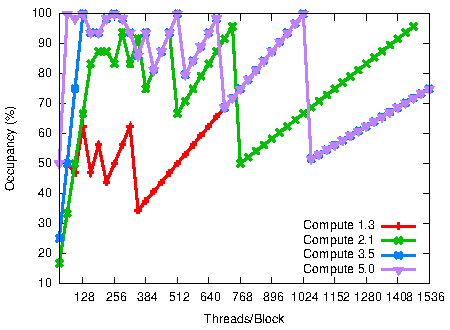
\includegraphics[width=0.8\textwidth]{images/sec-4/occupancy/occupancy}
    \caption[Impact of varying thread block size on multiprocessor occupancy]{
        Illustration of the impact of varying the thread block size on the
        overall multiprocessor occupancy. The example kernel requires 22
        registers per thread and 16 bytes of shared memory per thread. Each
        device generation (compute capability) achieves peak occupancy at
        different points in the sequence, so selecting a static thread block
        size for all kernels and devices is clearly suboptimal. Older devices
        are unable to achieve 100\% occupancy due to limitations in the register
        file size and available shared memory. The first two generations of
        devices can not execute the kernel with more than 704 and 1472 threads
        per block respectively.}
    \label{fig:occupancy}
\end{figure}


\subsection{Kernel execution}

To evaluate the array computation on the CUDA backend, we perform a bottom-up
traversal of the annotated program (\S\ref{sec:annotating_array_programs})
executing the attached kernels. For each node of the AST, we distinguish three
cases:
%
\begin{enumerate}
\item If it is a @Use@ node, return a reference to the device memory holding the
    array data.

\item If it is a non-skeleton node, such as a let binding or shape conversion,
    the evaluator executes the operation directly by adjusting the environment
    or similar as required.

\item If it is a skeleton node, memory is allocated to hold the result of
    evaluating the skeleton, and finally invokes the one or more GPU kernels
    that implement the operation.
\end{enumerate}
%
In summary, the execution pass interleaves host-side evaluation and the
invocation of GPU kernels, while keeping track of device memory, allocating
intermediates, and releasing memory once no longer required. See
section~\ref{sec:memory_management} for details on memory management. GPU
kernels execute asynchronously, so the evaluator is able to immediately begin to
set up the next stage of the computation while the current kernel executes. The
CUDA runtime maintains the sequence of kernels to be executed on the device,
known as the execution \emph{stream}.
% so if the result of an asynchronously executing kernel is needed before the
% kernel completes, any kernels that depend on that result will only be invoked
% after the kernel completes.

\subsection{Kernel execution, concurrently}

Beginning with compute capability 2.0, some CUDA devices are able to execute
multiple kernels concurrently, rather than always executing kernels one after
the other. This can improve overall performance by increasing the number of
active threads on the device, particularly when executing many small kernels.
Accelerate's collective operations have a purely functional semantics, so
concurrent expression evaluation is always sound. The current implementation
executes subtrees of the expression concurrently on the single device. We leave
for future work additionally executing programs concurrently on separate GPUs,
as is available in some Tesla configurations.

In order to execute kernels concurrently, the kernels must be issued in
different non-default streams. A \indexe{stream} is a sequence of commands that
execute in order; different streams, on the other hand, may execute their
commands out of order with respect to one another or concurrently. To allow
streams to synchronise, an \indexe{event} may be inserted into a stream. Any
stream may delay execution until a given event has been posted, which allows
efficient cross-stream synchronisation that is managed by the device.

The Accelerate CUDA backend introduces concurrency when evaluating the bound
expression at a let binding, and synchronises when looking up a bound variable
in the environment. Following conversion and optimisation of the program by the
Accelerate frontend, any operation that is to be evaluated will appear as a
let-bound expression in the program, and so sequences of let bindings may be
able to execute their subtrees concurrently. The array expression evaluator has
the type:
%
\begin{lstlisting}[style=haskell]
executeOpenAcc
    :: ExecOpenAcc aenv arrs            -- annotated array program (\S\ref{sec:annotating_array_programs})
    -> Aval aenv                        -- array environment with synchronisation points
    -> Stream                           -- current execution stream
    -> CIO arrs
\end{lstlisting}
%
The array environment is augmented to carry both the array object as well as an
event execution streams can synchronise against, which signals that the array
has been fully evaluated:
%
\begin{lstlisting}[style=haskell]
data Async a = Async Event a

data Aval env where
  Aempty :: Aval ()
  Apush  :: Aval env -> Async t -> Aval (env, t)
\end{lstlisting}

The only interesting cases for the evaluator are those of let bindings and
environment lookup. When looking up an array in the environment, we ensure that
all future work submitted to the current stream will occur after the
asynchronous event for the array in the environment has been fulfilled.
Synchronisation occurs on the device, so the following does not block waiting
for the result:
% \footnote{\footcode{Event.wait} is the FFI binding to \footcode{cudaStreamWaitEvent} and comes from the CUDA binding library.}
%
\begin{lstlisting}[style=haskell]
after :: Stream -> Async a -> CIO a
after stream (Async event arr) = Event.wait event (Just stream) [] >> return arr
\end{lstlisting}

Evaluating the binding of a let requires evaluating the expression in a new
asynchronous execution stream. The body expression is then evaluated with the
bound array wrapped in an @Async@, which contains the event indicating when the
last kernel issued to the stream has completed.
%
\begin{lstlisting}[style=haskell]
streaming :: Context
          -> Reservoir
          -> (Stream -> CIO a)
          -> (Async a -> CIO b)
          -> CIO b
streaming ctx rsv`(Reservoir _ weak_rsv) bnd body = do
    stream <- create ctx rsv                                                       -- (1)
    bnd'   <- bnd stream                                                           -- (2)
    end    <- Event.waypoint stream
    body'  <- body (Async end bnd')                                                -- (3)
    destroy (weakContext ctx) weak_rsv stream                                      -- (4)
    Event.destroy end
    return body'
\end{lstlisting}
%
\begin{enumerate}
\item The function @create@ allocates a new execution stream. It uses a
    technique similar to the @Nursery@
    (\S\ref{sec:memory_manager_implementation}) to reuse execution streams that
    are currently idle, taking an inactive stream from the @Reservoir@ if one is
    available, or allocating a new execution stream otherwise.
%
% \begin{lstlisting}[style=haskell]
% type RSV        = MVar ( HashTable CUDA.Context (FullList () Stream) )
% data Reservoir  = Reservoir RSV (Weak RSV)
% \end{lstlisting}

\item The bound expression is executed asynchronously, assigned to the new
    @Stream@.

\item The body of the expression is evaluated. The extended array environment
    includes the event @end@, which will be signalled once the result of the
    binding is available.

\item Unlike the implementation of the memory manager, events and streams never
    remain active outside the evaluation of an Accelerate program, so the stream
    and event associated with evaluating the binding are explicitly deallocated
    after evaluation of the body completes.

\end{enumerate}

At an example, Listing~\ref{lst:concurrent_kernels} contains an example program
that is able to execute the nine @map@ operations concurrently on devices of
compute capability 2.0 and greater. Note that, to keep the example simple,
fusion is disabled to prevent the @map@ operations from fusing into the @zip9@.
The corresponding execution trace from the NVIDIA Visual Profiler application is
shown in Figure~\ref{fig:concurrent_kernels}, which demonstrates each of the
@map@ operations executing in separate streams and overlapping with each other.

\begin{lstlisting}[style=haskell_float
    ,float
    ,label=lst:concurrent_kernels
    ,caption={[Example program that executes kernels concurrently]
        An example program that executes each of the \code{map} kernels
        concurrently, on devices of compute capability 2.0 and greater. Note
        that in order to keep the example simple, the displayed behaviour is
        only seen when fusion is disabled, to prevent the operations from being
        combined into a singel kernel.}]
loop :: Exp Int -> Exp Int
loop ticks = A.while (\i -> i <* clockRate * ticks) (+1) 0
  where
    clockRate   = 900000

concurrentTest :: Acc (Vector (Int,Int,Int,Int,Int,Int,Int,Int,Int))
concurrentTest
  = A.zip9 (A.map loop (use $ fromList Z [1]))
           (A.map loop (use $ fromList Z [1]))
           ...
\end{lstlisting}

\begin{figure}[tbp]
    \centering
    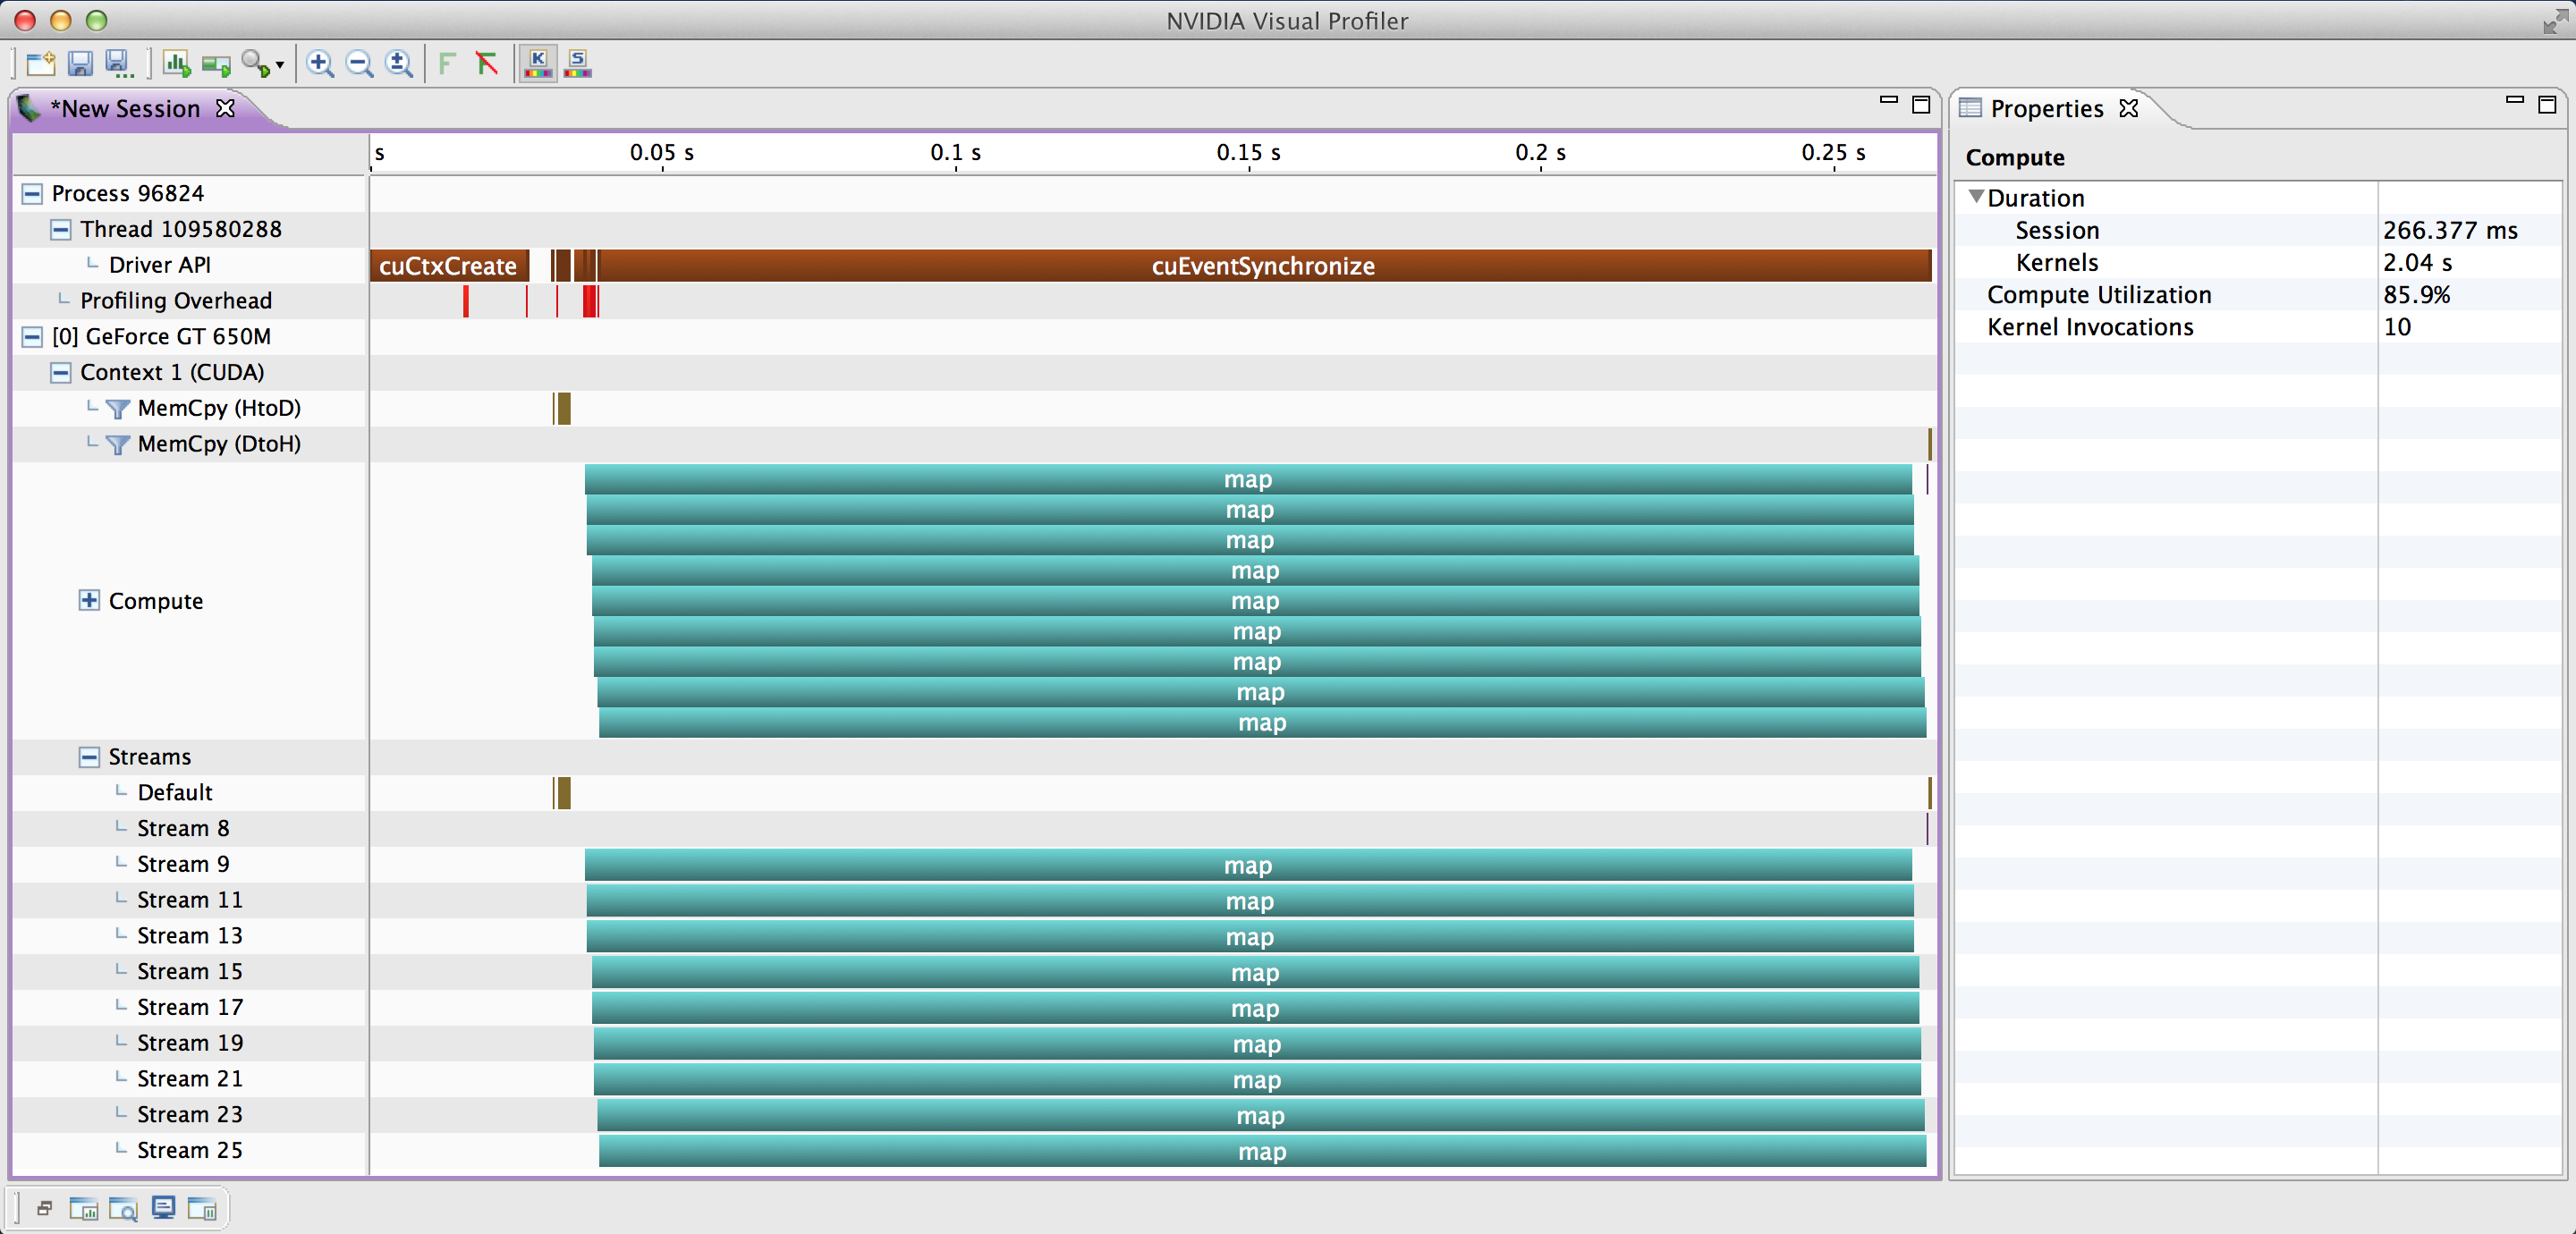
\includegraphics[width=\textwidth]{images/sec-4/concurrent_kernels}
    \caption[Profiling trace of a program which executes kernels
    concurrently]{Trace from the NVIDIA Visual Profiler application for the
    program shown in Listing~\ref{lst:concurrent_kernels}, where the nine
    \code{map} kernels execute concurrently on devices of compute capability 2.0
    and greater. Each \code{map} operation takes $226.7$~ms to execute. As
    shown, an equivalent of $2.04$~seconds of GPU time is execute in a wall
    clock time of $266.4$~ms, which includes program initialisation.}
    \label{fig:concurrent_kernels}
\end{figure}

\subsubsection{Interaction with Array Fusion}

In the example shown in Listing~\ref{lst:concurrent_kernels}, it was necessary
to disable the array fusion optimisation (\S\ref{sec:array_fusion}) in order to
prevent the kernels being combined into a single kernel, within which each of
the fused operations execute sequentially. While a simple example was chosen on
purpose in order to clearly demonstrate kernels executing concurrently, the same
situation nevertheless arises in real programs. That is, by combining sequences
of operations into a single operation, fusion has the effect of removing
opportunities for concurrent kernel execution.

It is left to future work to provide some analysis of when it would be
beneficial to avoid fusing operations, on the basis that it would be more
efficient to instead execute the two sub-computations concurrently. Such an
analysis would need to take into account the hardware that the program is to be
executed on, as well as an estimate of how much of the GPU's resources each
kernel requires. This is required in order to determine if the two kernels could
be scheduled concurrently.


\subsection{Conclusion}

Runtime system operations are important, as they partially compensate for the
overhead of being an embedded language; that is, of needing to traverse the
program AST in order to evaluate it. The Accelerate runtime system is designed
to execute programs as efficiently as possible, which in turn helps maximise the
computational utilisation of the device, and ensure all processors are kept
busy.

The runtime system attempts to optimise both individual kernel executions, as
well as execution of the entire program. In the former case, each kernel launch
is configured to maximise thread occupancy for the particular device the kernel
is being executed on, and kernels are scheduled such that independent operations
can be executed concurrently, on devices which support this. The single most
important optimisation, however, is that each node of the program AST is
decorated with all of the data required do execute that operation. For programs
which are executed more than once, this means that the costly front-end analysis
and code generation steps of program execution can be skipped on the second and
subsequent invocations of the program, and kernels can begin executing
immediately. This process happens automatically, and almost\footnote{The user
user must express their program in the form of a function of one array argument,
and use the corresponding \code{run1} function to execute the program. This is
not so onerous, as any operation that the user intends to execute multiple times
is likely to be easily written in the form of a function from arrays to arrays.}
entirely transparently to the user.

With these optimisations, the Accelerate runtime system is efficient enough that
we can execute numerically intensive programs such as fluid flow simulations
(\S\ref{sec:fluid}) and real-time image processing applications
(\S\ref{sec:canny}) and achieve performance comparable to hand-written CUDA
programs.


\section{Related work}
\label{sec:implementation_related}

The development of general-purpose applications that run on the GPU is highly
work intensive, and has been estimated to require at least $10\times$ as much
effort as developing an efficient single-threaded
application~\cite{Sweeney:2009ua}. Several researchers have proposed to
ameliorate the status quo by either using a high-level library to compose GPU
code or by compiling a subset of a high-level language to low-level GPU code.
This section explores some of these approaches.


\subsection{Embedded languages}

%% Haskell-based approaches

Vertigo~\cite{Elliott:2004hh} is an embedded language in Haskell for GPGPU
programming. Vertigo is a statically compiled graphics language targeting the
DirectX 8.1 shader model, and does not offer higher-order combinators such as
@map@ and @fold@.

Obsidian~\cite{Svensson:2008a} and Nikola~\cite{Mainland:2010vj} are also
Haskell EDSLs for GPGPU programming, and are in aim and spirit the embeddings
closest to Accelerate. Both Nikola and Obsidian produce CUDA code as we do,
however while we use algorithmic skeletons (\S\ref{sec:code_generation}), Nikola
explicitly schedules loops, and Obsidian is a lower level language where more
details of the GPU hardware are exposed to the programmer. Moreover, the
Accelerate language is more expressive, supporting generative functions such as
@replicate@, and Accelerate computations can span multiple GPU kernels, whereas
both Nikola and Obsidian can only express array computations that can be
implemented in a single GPU kernel. Algorithms spanning multiple kernels need to
be explicitly scheduled by the application programmer and incur additional
host-device data transfer overhead, which can be rather significant.

% \marginnote{tk: to related work for fusion?}
% Recent versions of Obsidian~\cite{Claessen:2012hl} implement
% Repa-style~\cite{Keller:2010er} delayed \emph{pull arrays} as well as \emph{push
% arrays}. Whereas a pull array represents a general producer, a push array
% represents a general consumer. Pull arrays allow intermediate programs to be
% written in continuation passing style (CPS)\index{continuation passing style},
% which helps to compile (and fuse) append-like operations.

Paraiso~\cite{Muranushi:2012eh} is a Haskell EDSL for solving systems of
\indext{partial differential equation}s (PDEs), such as hydrodynamics equations,
and generates both CUDA code for GPUs as well as OpenMP~\cite{OpenMP:2008} code
for multicore CPUs. Accelerate supports @stencil@ operations for expressing this
type of operation, but currently lacks a backend for multicore CPUs. Paraiso
also includes an automated tuning framework to search for faster implementations
of the algorithm.

Baracuda~\cite{Larsen:2011fa} is a Haskell EDSL producing CUDA GPU kernels,
though it is intended to be used offline, with the kernels called directly from
a C++ application. It supports only @map@ and @fold@ operations.


\subsection{Parallel libraries}

%% C++-based approaches

Accelerator~\cite{Bond:2010bd,Tarditi:2006} is a C++ library-based approach with
less syntactic sugar for the programmer, but bindings to functional languages.
In contrast to our current work, it already targets multiple architectures,
namely GPUs, FPGAs, and multicore CPUs. However, the code generated for GPUs
uses the DirectX 9 API, which does not provide access to several modern GPU
features, negatively impacting performance and preventing some operations such
as scatted writes.

RapidMind~\cite{LinXu:2008ig}, which targets the GPU using OpenCL, and its
predecessor Sh~\cite{McCool:2004,McCool:2004un} which used pixel shaders of the
graphics API, are C++ meta programming libraries for data parallel programming.
RapidMind was merged into Intel's Ct compiler to create the Array Building
Blocks (ArBB) library. However, the ArBB project was retired before support for
GPUs was integrated. GPU++~\cite{Jansen:2008vw} is an embedded language in C++
using similar techniques to RapidMind and Sh, but provides a more abstract
interface than the other C++ based methods listed here.

Thrust~\cite{ThrustAParallelT:ub} is a library of algorithms written in CUDA,
with an interface similar to the C++ Standard Template Library.
\citet{Sato:2009cq} describe a C++ library for GPGPU programming based on
algorithmic skeletons. Both of these libraries can be used to generate both CUDA
code for the GPU as well as OpenMP code targeting multicore CPUs.


%% other approaches

Dandelion~\cite{Rossbach:2013bj} is a library of data-parallel operations,
specified as comprehensions on arrays using the LINQ framework for .NET
(programmers write in either C@#@ or F@#@). Operations are compiled for the GPU
as well as the CPU, and the runtime system distributes the computation over all
of the available processors in a heterogeneous cluster.


PyCUDA~\cite{Klockner:2012tj} uses Python as a host language to provide access
to the low level CUDA driver API and to facilitate runtime code generation for
the GPU. A similar approach is taken by CLyther~\cite{CLyther:EvXSiruK} which
targets OpenCL. Copperhead~\cite{Catanzaro:2011cn} uses PyCUDA and Thrust
internally to provide a higher level of abstraction to compile, link, cache, and
execute CUDA code. Both Parakeet~\cite{Rubinsteyn:2012ve} and Anaconda
Accelerate~\cite{AnacondaAccelerate:2013vn} are Python libraries that attempt to
just-in-time compile a subset of Python code that uses the
NumPy~\cite{NumPy:2006uq} array library to instead target the GPU.

The Jacket~\cite{AccelerEyes:vq} extension to Matlab supports offloading matrix
computations to GPUs by introducing new datatypes for matrices allocated in GPU
device memory, and overloading existing operations so that operations on these
matrices triggers execution of suitable GPU kernels.


\subsection{Other approaches}

Delite/LMS~\cite{Rompf:2013er} is a parallelisation framework for DSLs in Scala,
and has several backend targets including CPUs and GPUs.

NDP2GPU~\cite{Bergstrom:2012bi} compiles NESL~\cite{Blelloch:1995ut} code to
CUDA. Performance suffers because the implementation relies on the legacy NESL
compiler, which produces a significant number of intermediate computations.

NOVA~\cite{Collins:2013wn} is a high-level lisp-like functional language and
compiler for parallel operations, targeting both GPUs and CPUs. Compared to
Accelerate, NOVA supports fewer parallel operations, but does claim to support
nested parallelism, recursion, and sum data types. The NOVA compiler has not
been released.


\section{Discussion}

This chapter has detailed the implementation of the Accelerate language and the
CUDA generating backend targeting parallel execution on NVIDIA GPUs. We
discussed our approach to skeleton-based code generation, as well as the caching
mechanisms that are implemented in order to reduce the overheads of the
embedding, such as of runtime code generation and compilation. This chapter also
dealt with the issue of memory management and data transfer, which is a key
consideration to achieving high performance. Finally, we discussed the execution
of the generated GPU kernels, including launch configuration and concurrent
execution optimisations, in order to maximise device utilisation and help reduce
overall program run times.

Now that we can compile and run Accelerate programs on the GPU, the next chapter
covers how to optimise Accelerate programs. In particular, we introduce our
type-safe approaches to sharing recovery and array fusion, which we identify as
the two most pressing performance limitations.


% \marginnote{perhaps split differently: real vs. embedded languages?}
% 
% Other significant parallel or GPGPU programming models and languages.
% Limitations that we share/avoid. Where we differ
% \begin{itemize}
% \item Repa \cite{Keller:2010er,Lippmeier:2011cd,Lippmeier:2012gx} (Haskell)
% \item SkeTo \cite{Matsuzaki:2011ew} (C++)
% \item list homomorphism based \cite{Sato:2009cq} (C++)
% \item Delite/LMS \cite{Rompf:2013er} (Scala)
% \item NDP2GPU \cite{Bergstrom:2012bi} (Haskell)
% \item Nikola \cite{Mainland:2010vj} (Haskell)
% \item Obsidian \cite{Svensson:2008a,Claessen:2012hl} (Haskell)
% \item Baracuda \cite{Larsen:2011fa} (Haskell)
% \item Jacket/ArrayFire \cite{AccelerEyes:vq} (Matlab)
% \item Anaconda Accelerate \cite{AnacondaAccelerate:2013vn} (Python)
% \item NOVA \cite{Collins:2013wn} (lisp)
% \item Dandelion \cite{tk} (LINQ)
% \end{itemize}



%
% END
%

%\begin{itemize}
%\item implementing parallel algorithms (20\%, 1 week)
%    \begin{itemize}
%        \item fold
%        \item scan
%        \item permute (atomic operations)
%        \item segmented/rank polymorphic operations
%    \end{itemize}
%
%\item skeleton-based code generation (2 weeks)
%    \begin{itemize}
%        \item device capabilities (free array variables, @umul24@,
%            @shfl@, atomic operations, shared memory)
%        \item rank polymorphic operations
%    \end{itemize}
%
%\item runtime system (3 weeks)
%    \begin{itemize}
%        \item launching kernels (occupancy calculator)
%        \item caching compiled kernels (live \& persistent caches)
%        \item memory management (escaping the EDSL evaluator; weak pointers vs.
%            reference counting)
%        \item executing kernels (annotated AST)
%    \end{itemize}
%
%\end{itemize}

% \begin{itemize}
%\item Accelerate frontend
%    \begin{itemize}
%        \item reification
%            \begin{itemize}
%                \item smart constructors for type classes
%                \item explicit dictionaries (polymorphism)
%                \item environments
%                \item HOAS vs. de Bruijn
%                \item representation types
%            \end{itemize}
%        \item surface \& internal (core) languages
%            \begin{itemize}
%                \item representing different constructs in surface/core
%                \item surface nested $\rightarrow$ core flat ?? (fuuuuture)
%            \end{itemize}
%        \item sharing observation ( --> sec 5? not my work )
%    \end{itemize}
%
%\item Accelerate CUDA backend
%    \begin{itemize}
%        \item code generation
%            \begin{itemize}
%                \item architecture sensitive JIT cross-compiler
%                \item future work: types, Haskell compile time
%            \end{itemize}
%        \item external compilation
%            \begin{itemize}
%                \item annotating AST nodes
%            \end{itemize}
%        \item memory management
%            \begin{itemize}
%                \item weak pointers \& weak hash tables
%                \item advantages to alternatives
%            \end{itemize}
%        \item execution
%            \begin{itemize}
%                \item occupancy analysis
%                \item multi-pass kernels
%            \end{itemize}
%        \item performance
%            \begin{itemize}
%                \item amortizing overheads (how to quantise this?)
%                \item of generated code
%                \item runtime overheads
%                \item w.r.t. CUDA memory subsystem (theoretical performance)
%                \item examples! spot the infelicities! (dot product)
%            \end{itemize}
%    \end{itemize}
%\end{itemize}

%Compilation has five phases:
%\begin{itemize}
%    \item Lexing
%    \item Parsing
%    \item Semantic analysis
%    \item Optimisation
%    \item Code Generation
%\end{itemize}

% EDSL basics:
%
% http://www.haskell.org/haskellwiki/Embedded_domain_specific_language
% http://www.haskell.org/haskellwiki/Research_papers/Domain_specific_languages
% 
% There are two major degrees of embedded languages:
% 
% \begin{description}
% \item[Shallow:] Operations immediately translate into the target language.
% 
% \item[Deep:] Operations build a data-structure that reflects the expression to
%     be evaluated. This structure allows the expression to be transformed before
%     being translated into the target language; for example by applying
%     optimisations.
% \end{description}
% 
% Sharing and recursion are common problems when implementing embedded domain
% specific languages.
